\section{はじめに}
\subsection{開発の目的}
本レポートでは，Webアプリケーション開発の基礎技術習得を目的として作成したシステムについて報告する．
近年のWebシステムにおいて不可欠な技術である，サーバサイドでの動的なコンテンツ生成を実現するNode.jsおよびExpressフレームワークを利用し，データの「新規登録（Create）」「一覧，詳細表示（Read）」「編集・更新（Update）」「削除（Delete）」という基本機能（CRUD）を備えたアプリケーションを構築した．
本開発では，操作性や画面遷移を統一した3つの異なるシステムを作成することで，データ構造が異なっても共通の設計思想で実装可能であることを確認した．

\subsection{作成したシステム}
本課題では，以下の3つのシステムを作成した．
\begin{enumerate}
    \item \textbf{成績管理システム}：履修した科目の単位数や成績を記録し，学修状況を管理するシステム．
    \item \textbf{教員情報システム}：所属学科や職位，担当科目などの教員情報を一元管理し，閲覧するシステム．
    \item \textbf{お小遣い帳システム}：日々の支出を記録し，合計金額を自動計算して表示する金銭管理システム．
\end{enumerate}



\section{利用者向けドキュメント}
本節では，作成したシステムのうち「お小遣い帳システム」を例に，利用方法について説明する．なお，他の2つのシステムについても操作方法は統一されており，同様の手順で利用可能である．

\subsection{概要}
本システムを利用するためには，Google ChromeやMicrosoft EdgeなどのWebブラウザが必要である．また，システムを利用する前に，管理者によってWebサーバが起動されている必要がある．
お小遣い帳システムでは，日々の買い物の「日付」「項目」「値段」などを記録し，一覧画面で支出の合計を確認することができる．

\subsection{起動画面（メインメニュー）}
Webブラウザのアドレスバー（図\ref{fig:URL}）に \url{http://localhost:8080/} と入力してアクセスすると，メインメニューが表示される（図\ref{fig:top}）．
ここから「お小遣い帳」のリンクをクリックすることで，お小遣い帳システムへ移動できる．万が一，存在しないページへアクセスした場合は「ページが見つかりません」と表示され，トップページへ戻るリンクが提供される（図\ref{fig:404}）．

\begin{figure}[H]
 \begin{center}
  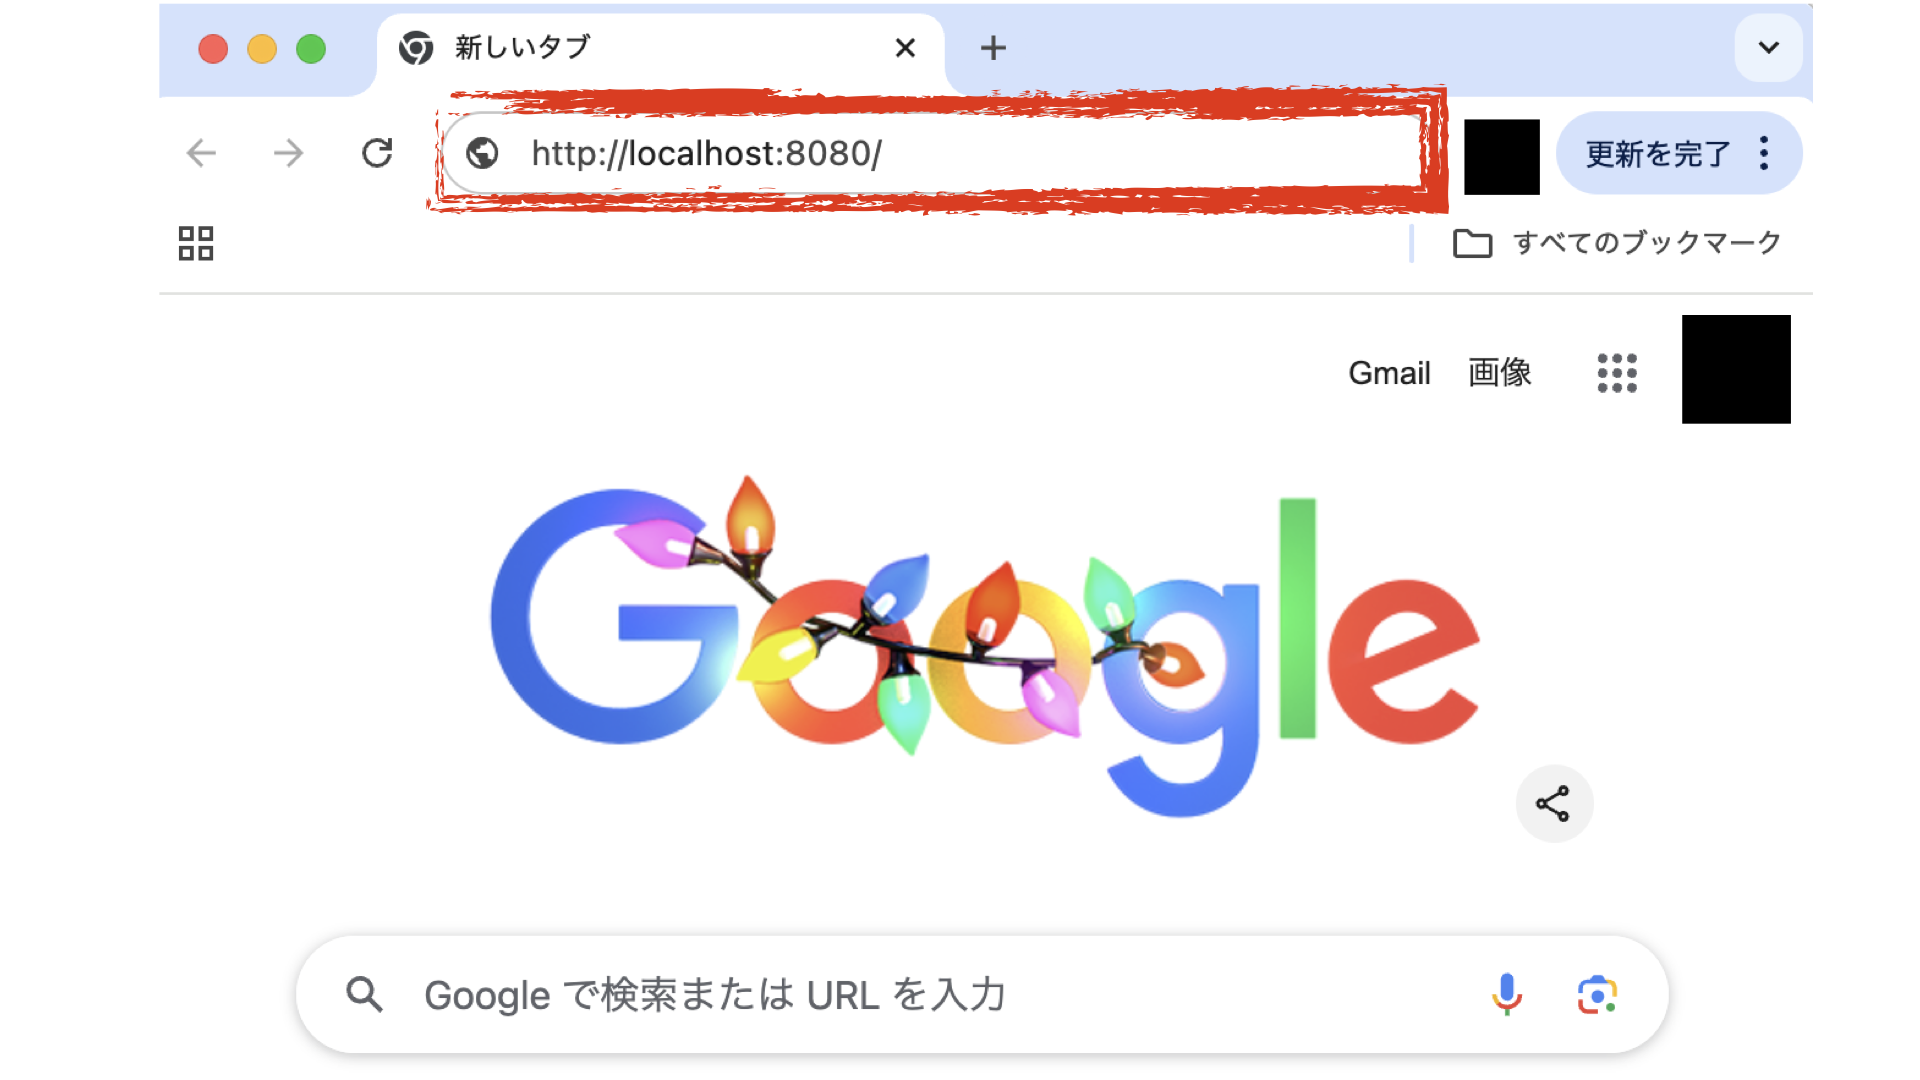
\includegraphics[width=13cm]{fig_web/URL.png}
  \caption{Google Chromeの場合のアドレスバーの位置}
  \label{fig:URL}
 \end{center}
\end{figure}
\begin{figure}[H]
 \begin{center}
  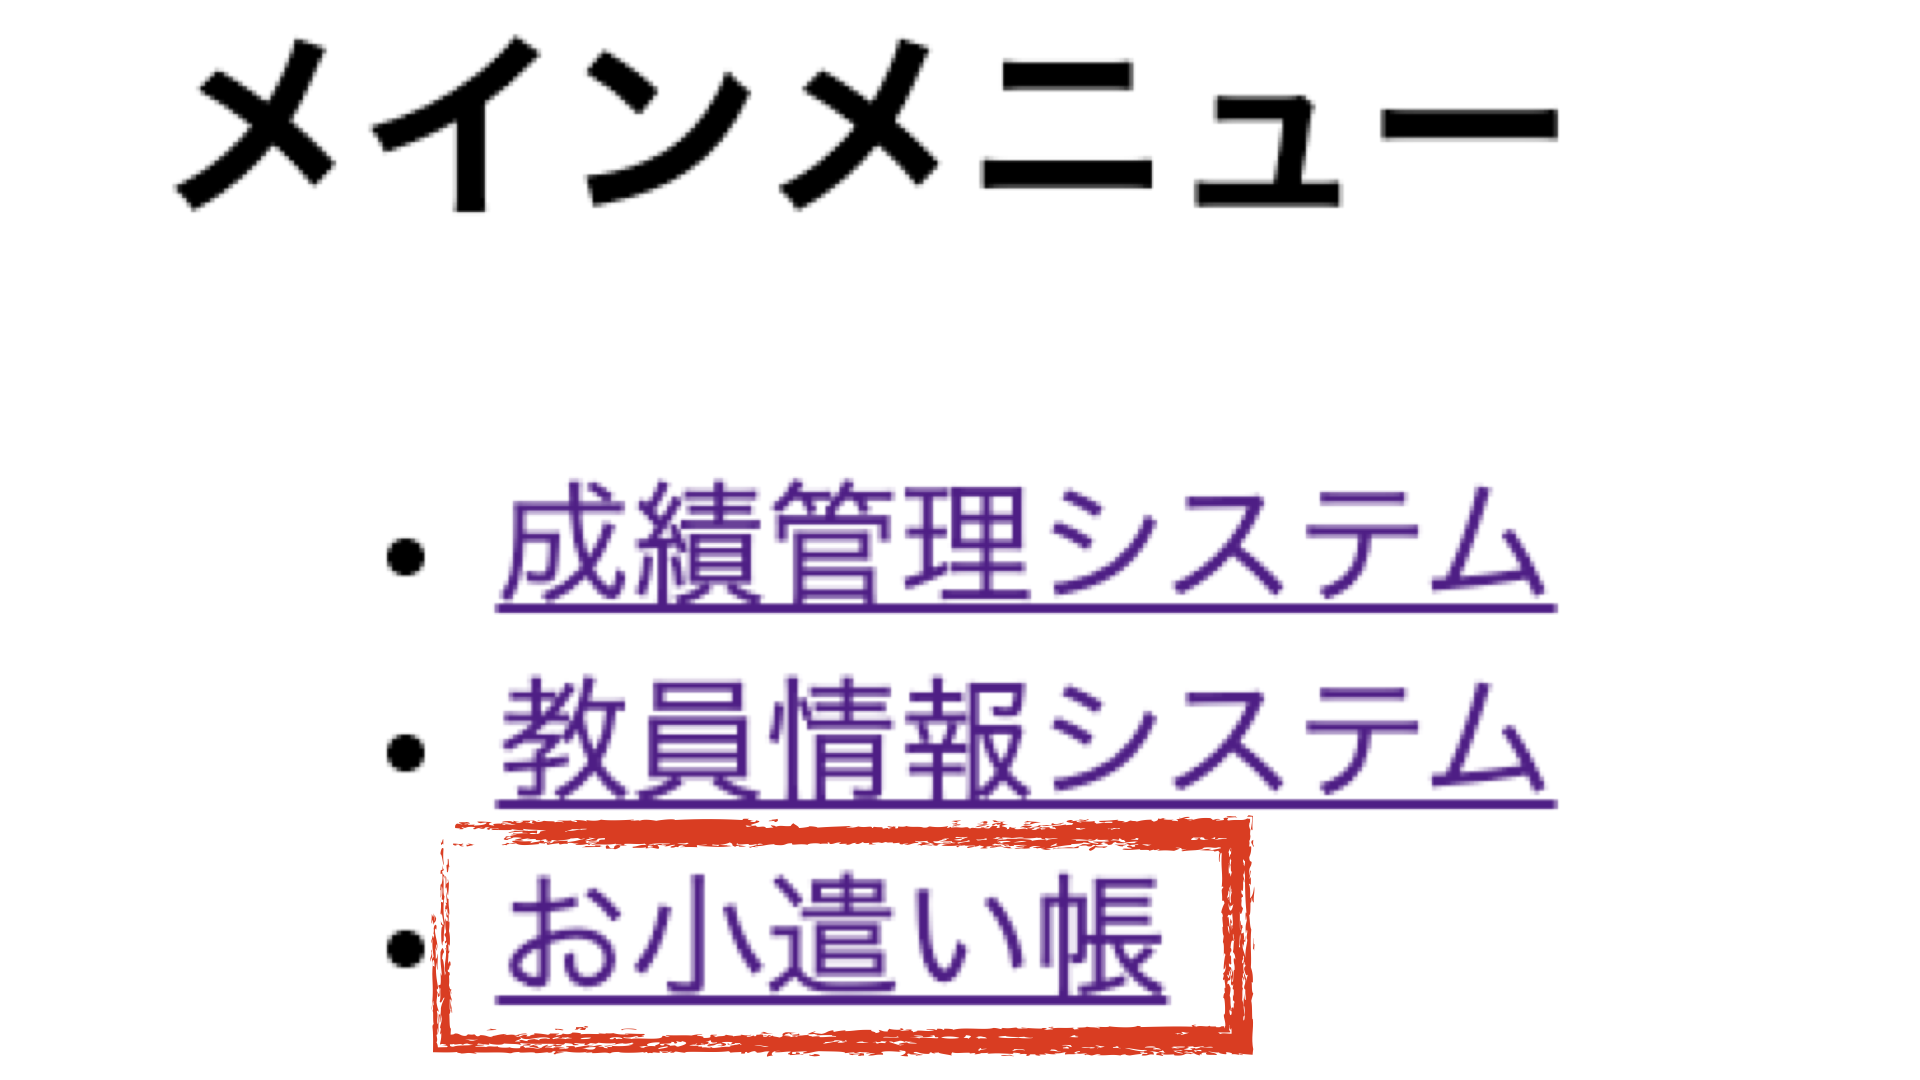
\includegraphics[width=5cm]{fig_web/top.png}
  \caption{メインメニュー画面}
  \label{fig:top}
 \end{center}
\end{figure}
\begin{figure}[H]
 \begin{center}
  
\includegraphics[width=5cm]{fig_web/404.png}
  \caption{存在しないページへアクセスした場合の画面}
  \label{fig:404}
 \end{center}
\end{figure}

\subsection{一覧表示}
お小遣い帳システムにアクセスすると，現在登録されているデータの一覧が表示される（図\ref{fig:list}）．
表には「日付」「項目」「値段」が表示され，表の最下部には登録されている全データの合計金額が自動計算されて表示される．
各項目のリンクをクリックすると，そのデータの詳細画面へ遷移する．

\begin{figure}[H]
 \begin{center}
  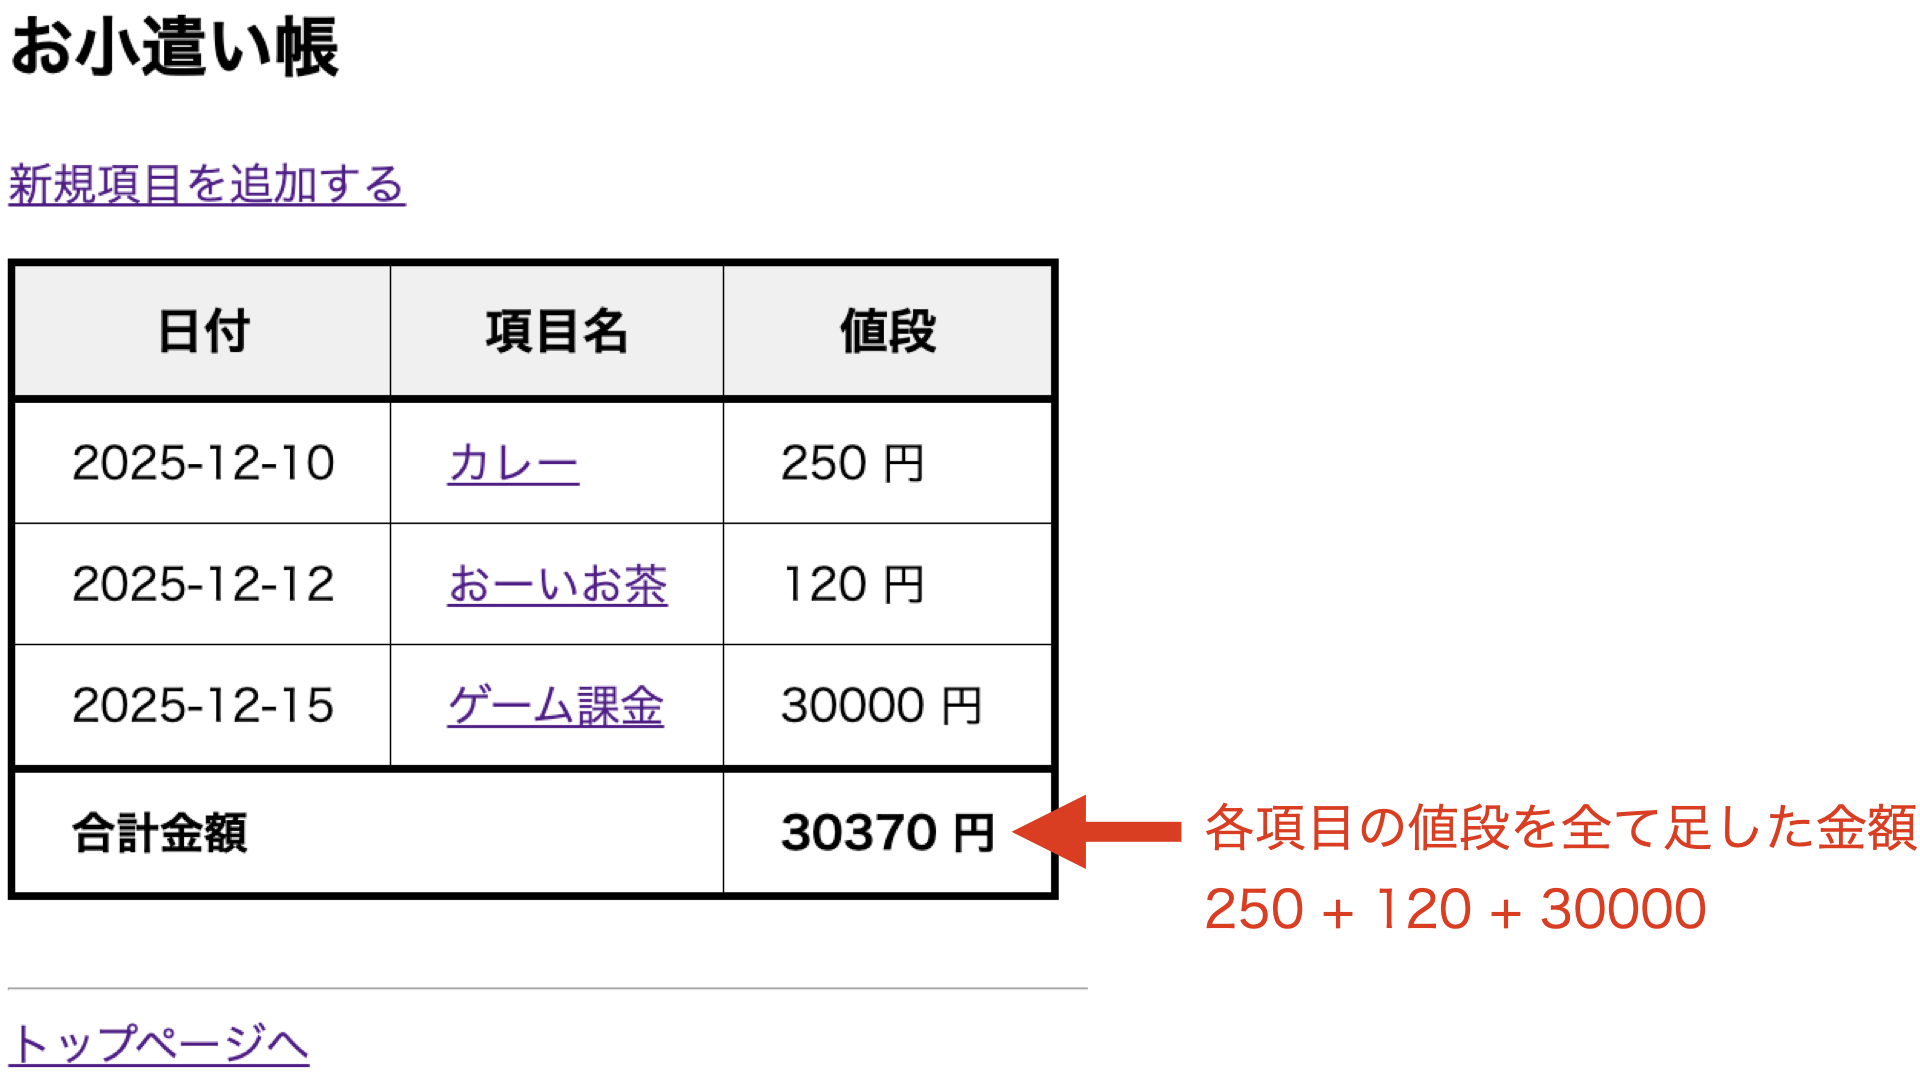
\includegraphics[width=13cm]{fig_web/wallet_list.png}
  \caption{お小遣い帳の一覧表示画面（合計金額が表示される）}
  \label{fig:list}
 \end{center}
\end{figure}

\subsection{詳細表示}
一覧画面で項目名をクリックすると，詳細表示画面へ遷移する（図\ref{fig:detail}）．
ここでは，一覧には表示しきれなかった「購入目的」や「備考欄」を含むすべての情報を確認できる．
また，この画面からデータの「編集」や「削除」を行うためのリンクが配置されている．

\begin{figure}[H]
 \begin{center}
  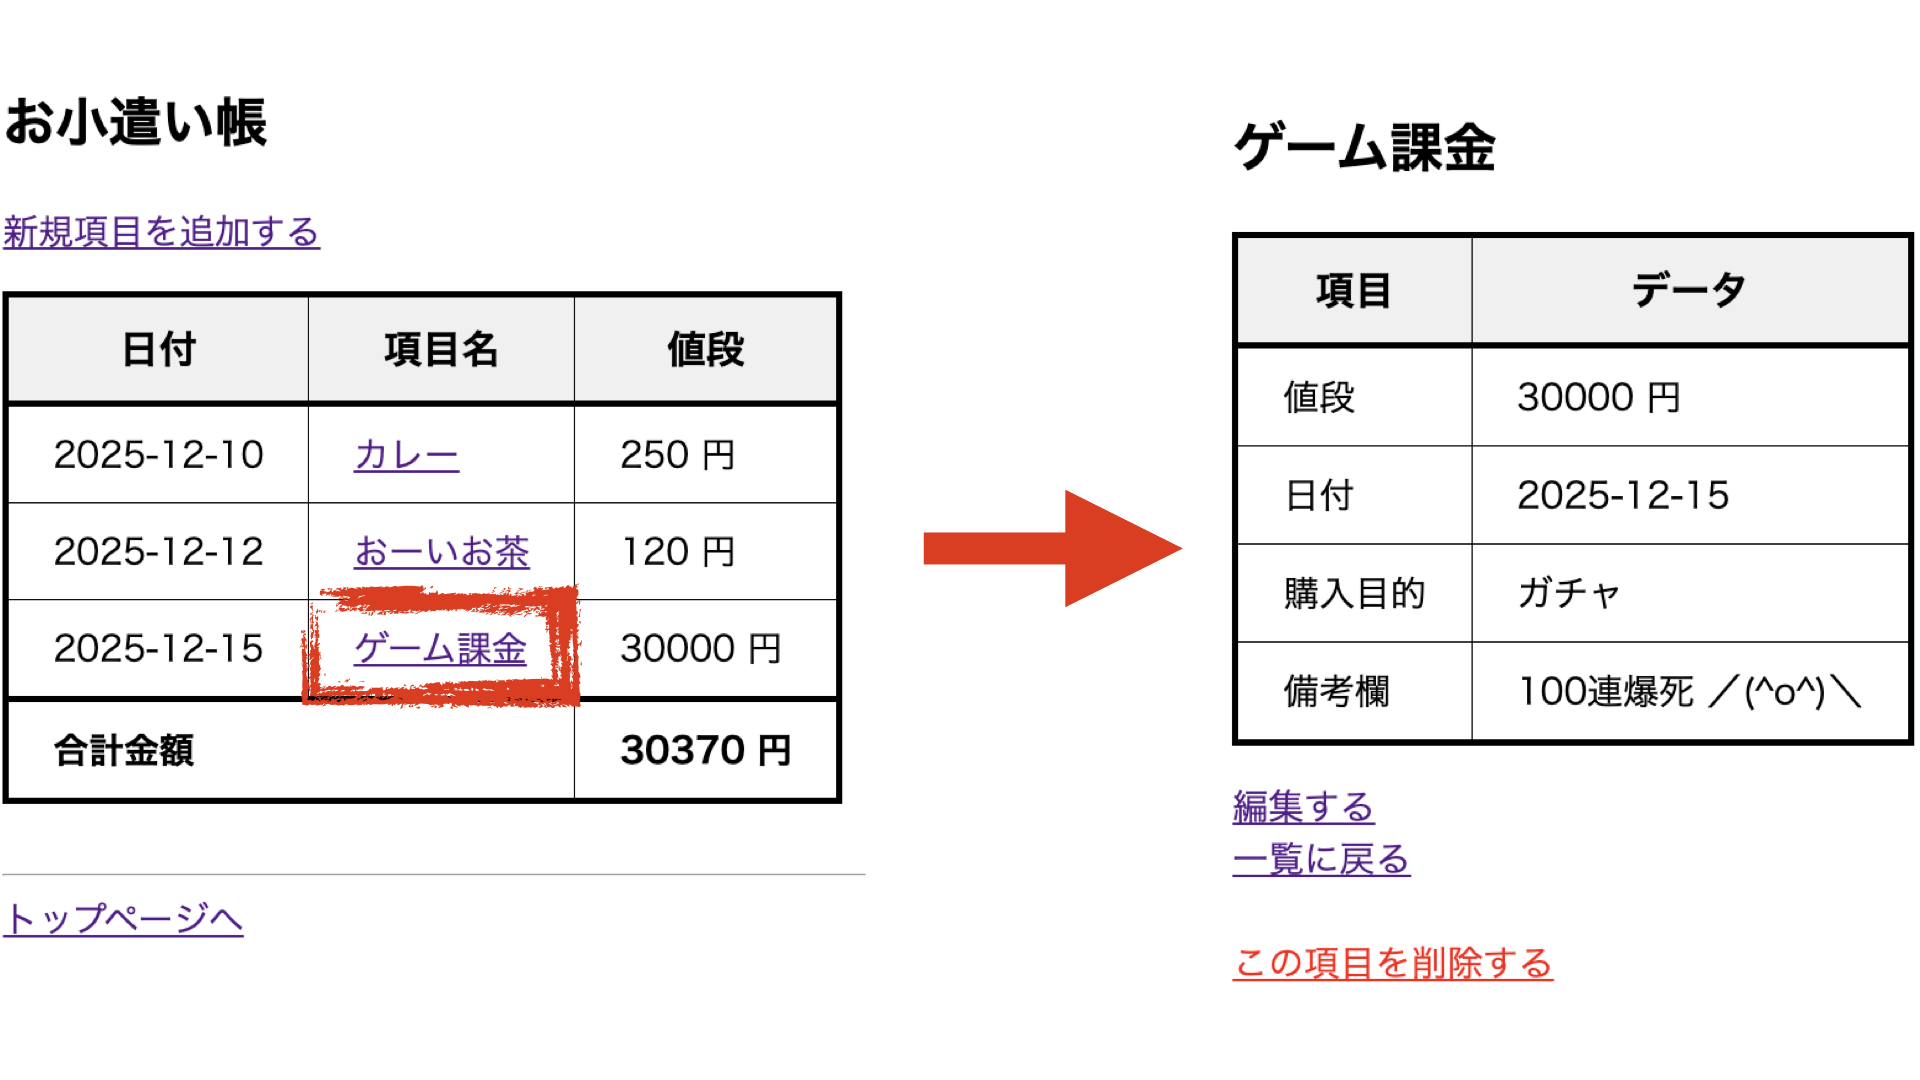
\includegraphics[width=15cm]{fig_web/wallet_detail.png}
  \caption{詳細表示の内容と仕方}
  \label{fig:detail}
 \end{center}
\end{figure}

\subsection{データの編集}
登録済みのデータを修正する手順は以下の通りである．
\begin{enumerate}
    \item 修正したいデータの詳細画面を開き，「編集する」リンクをクリックする（図\ref{fig:go_to_edit}）．
        \begin{figure}[H]
        \begin{center}
        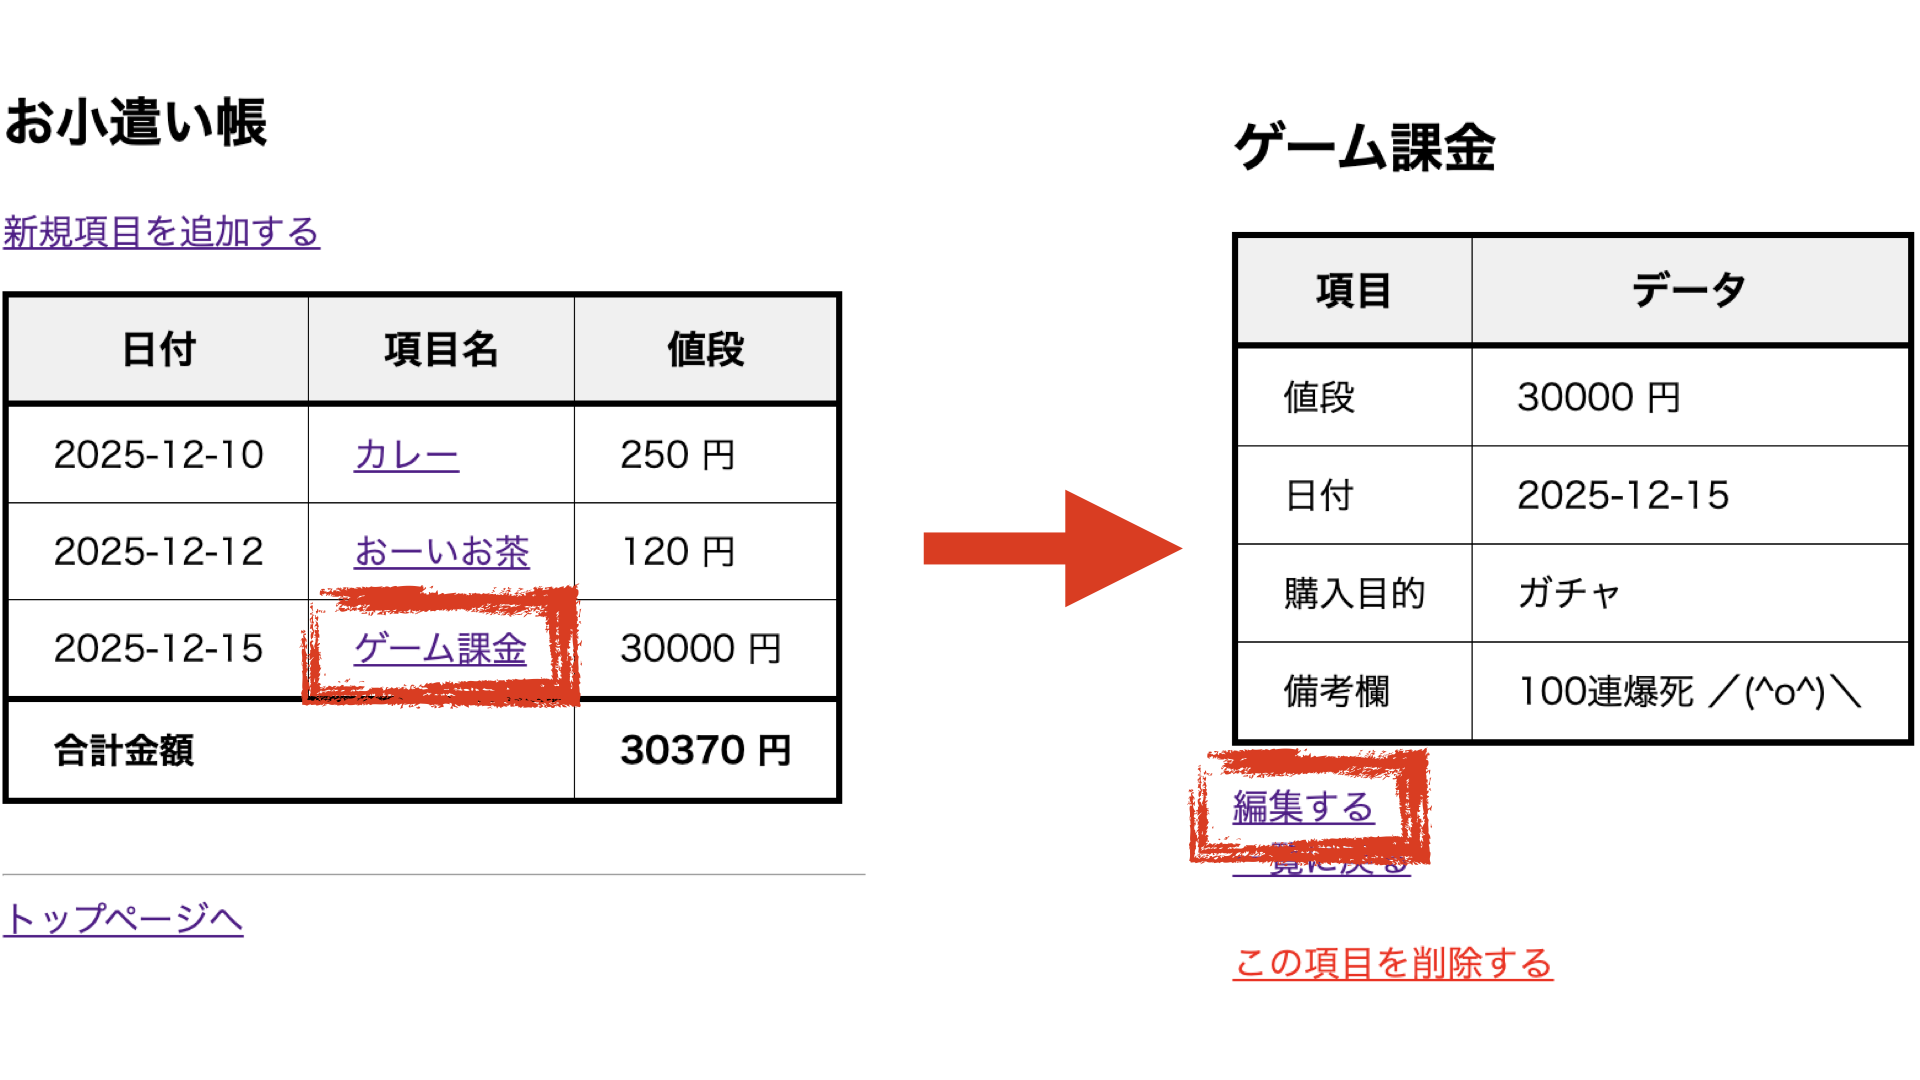
\includegraphics[width=15cm]{fig_web/wallet_go_to_edit.png}
        \caption{編集画面への行き方}
        \label{fig:go_to_edit}
        \end{center}
        \end{figure}
    \clearpage
    \item 編集画面が表示される（図\ref{fig:edit}）．現在のデータが入力欄に入った状態で表示されるため，修正したい箇所のみ書き換える．
        \begin{figure}[H]
        \begin{center}
        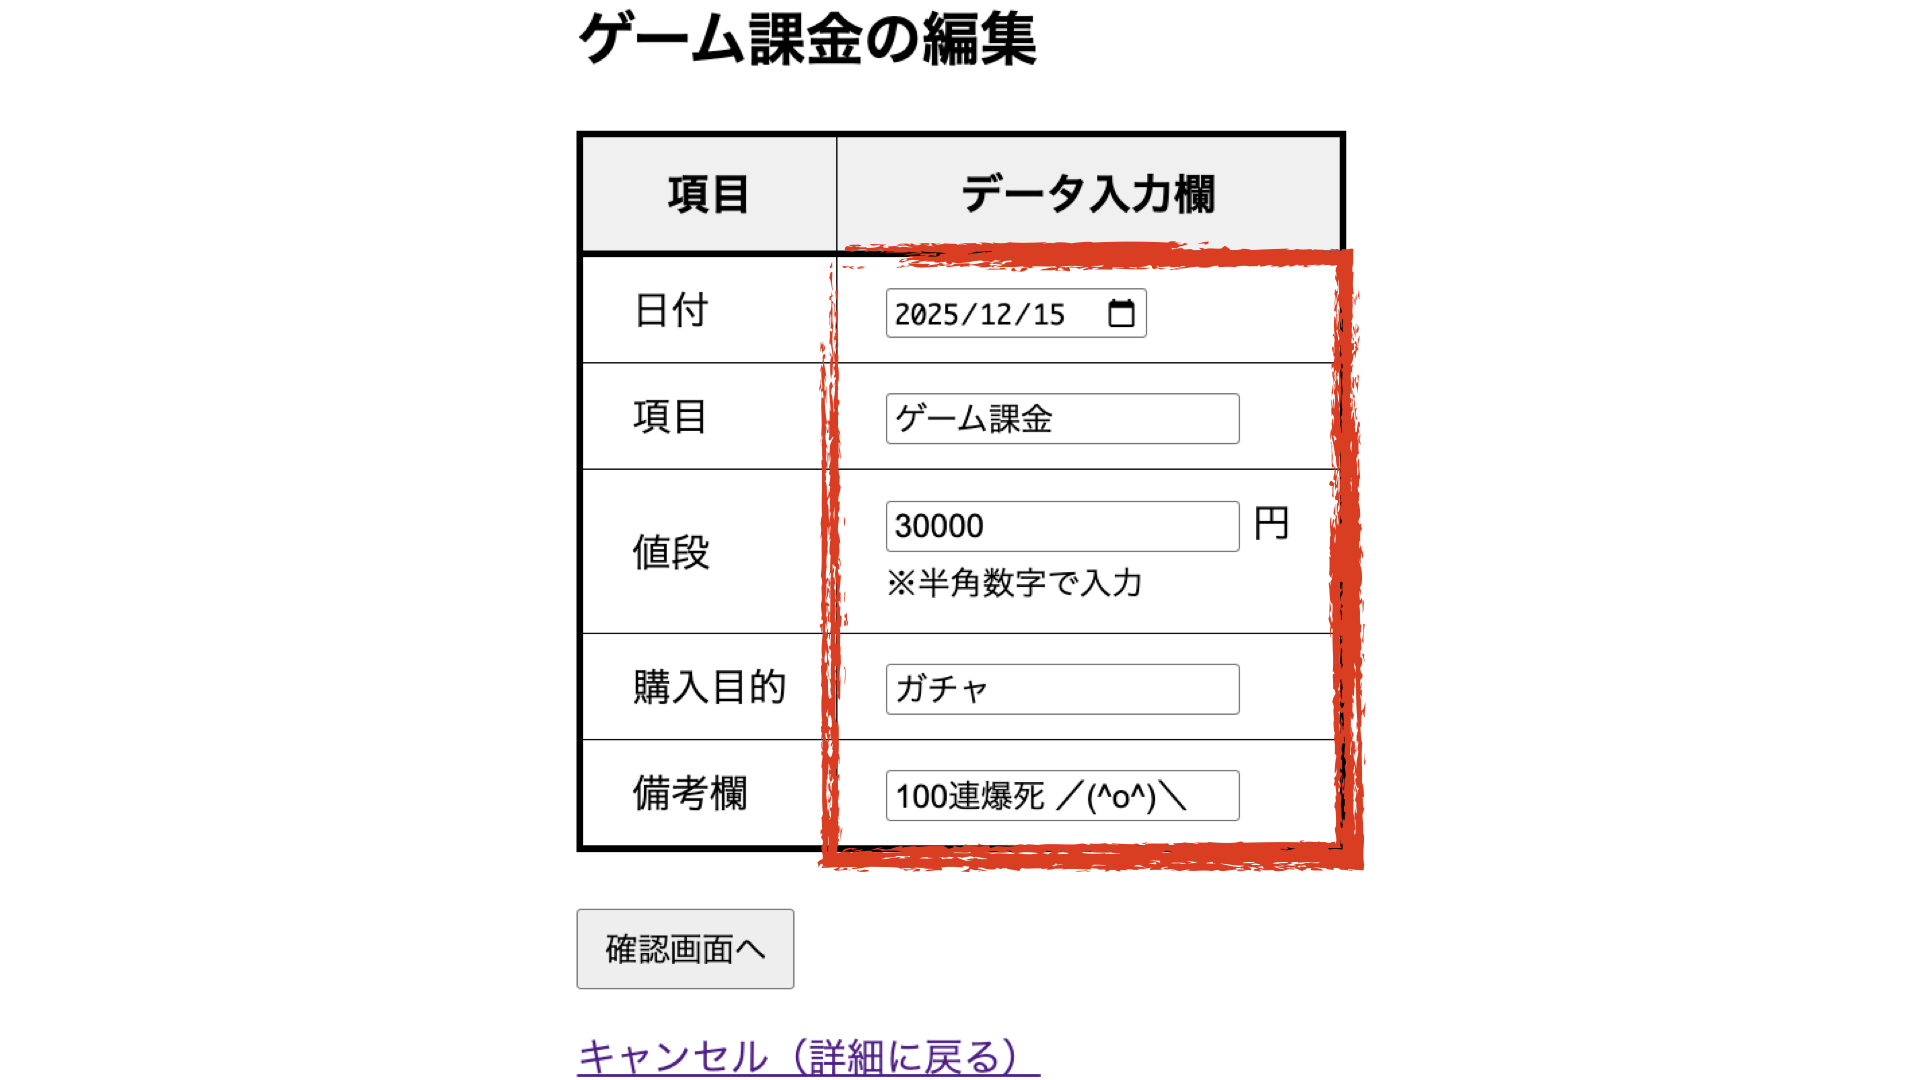
\includegraphics[width=15cm]{fig_web/wallet_edit.png}
        \caption{編集画面}
        \label{fig:edit}
        \end{center}
        \end{figure}
    \item 修正が完了したら「確認画面へ」ボタンを押す（図\ref{fig:edit_change}）．
        \begin{figure}[H]
        \begin{center}
        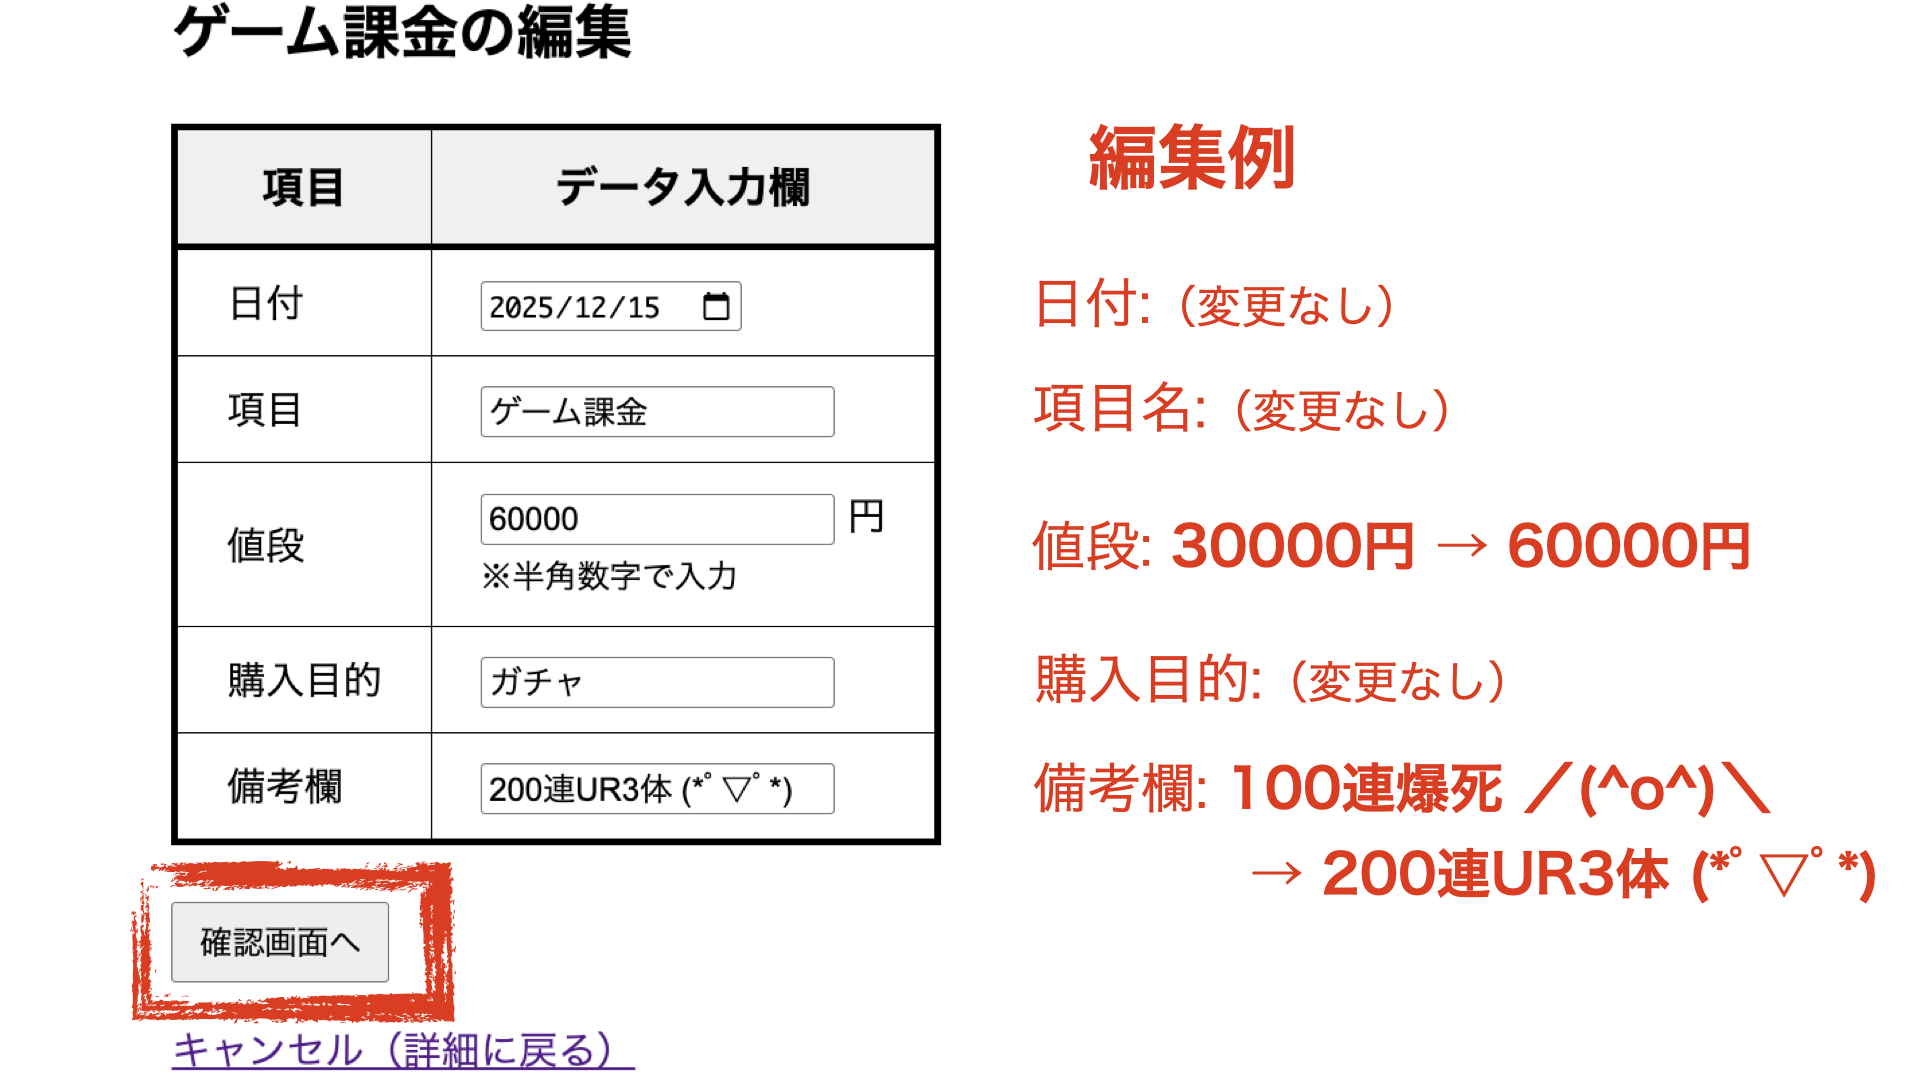
\includegraphics[width=15cm]{fig_web/wallet_edit_change.png}
        \caption{編集例と「確認画面へ」ボタン}
        \label{fig:edit_change}
        \end{center}
        \end{figure}
    \clearpage
    \item 表示された確認画面で変更内容を確認する（図\ref{fig:edit_confirm}）．修正が必要な場合は「修正する」ボタンを押して編集画面へ戻る．
        \begin{figure}[H]
        \begin{center}
        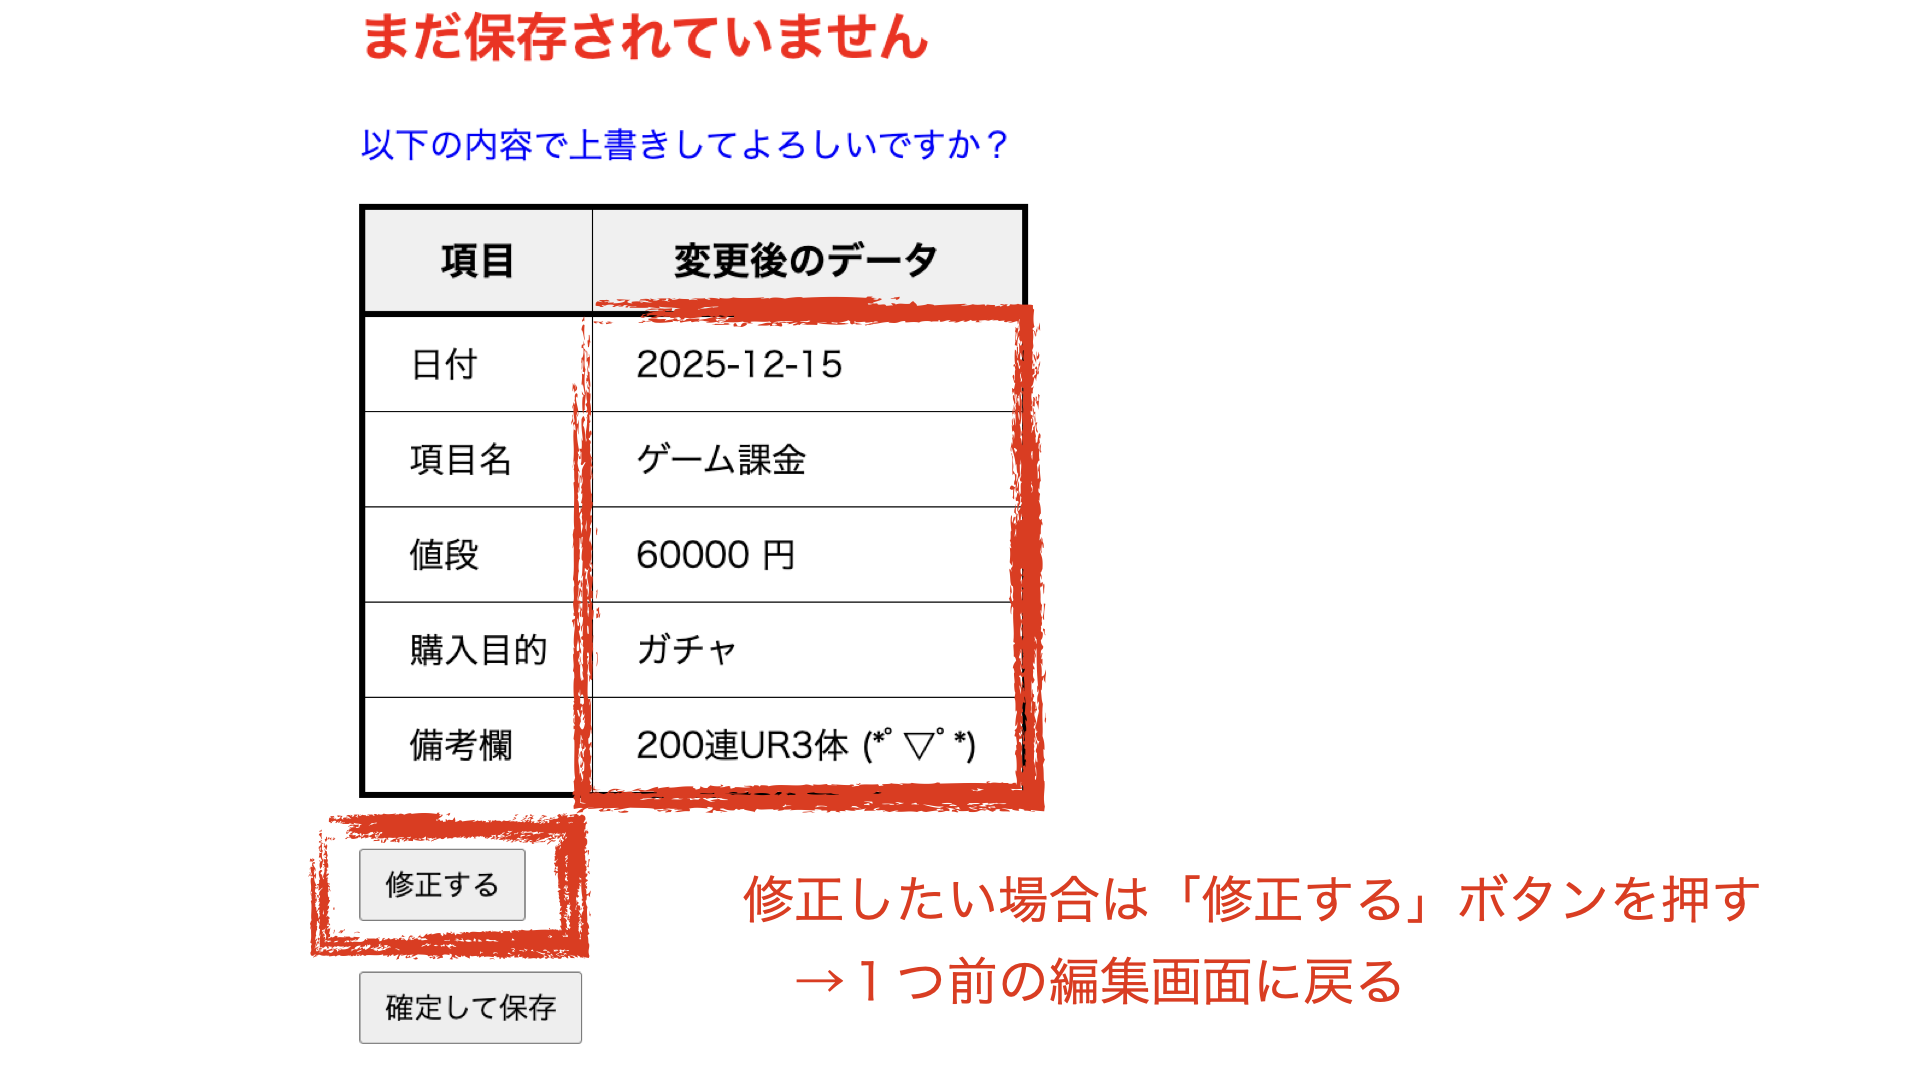
\includegraphics[width=15cm]{fig_web/wallet_edit_confirm.png}
        \caption{編集内容確認画面}
        \label{fig:edit_confirm}
        \end{center}
        \end{figure}
    \item 「確定して保存」ボタンを押すと，データが上書き保存され，詳細画面へ戻る（図\ref{fig:edit_fin1}）．一覧表示にも変更が反映されている（図\ref{fig:edit_fin2}）．
        \begin{figure}[H]
        \begin{center}
        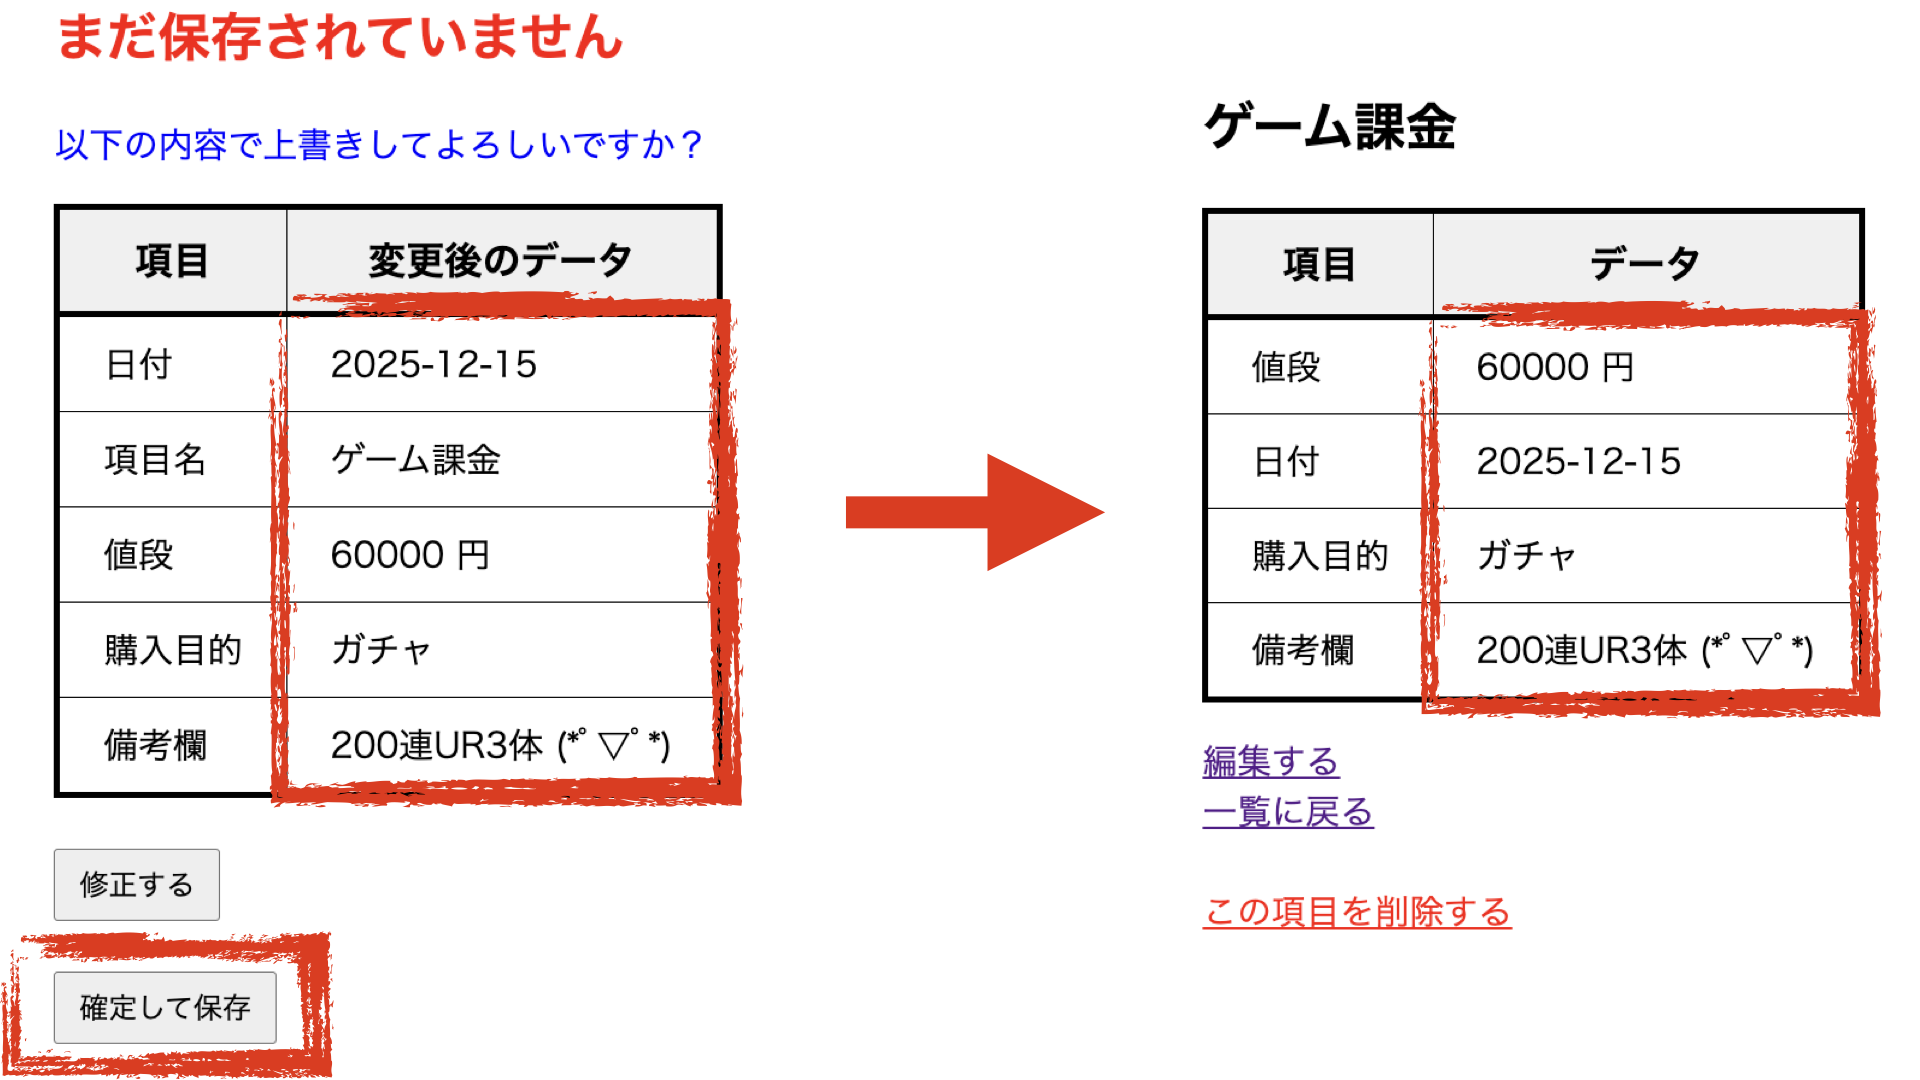
\includegraphics[width=15cm]{fig_web/wallet_edit_fin1.png}
        \caption{編集完了後の画面}
        \label{fig:edit_fin1}
        \end{center}
        \end{figure}
        \begin{figure}[H]
        \begin{center}
        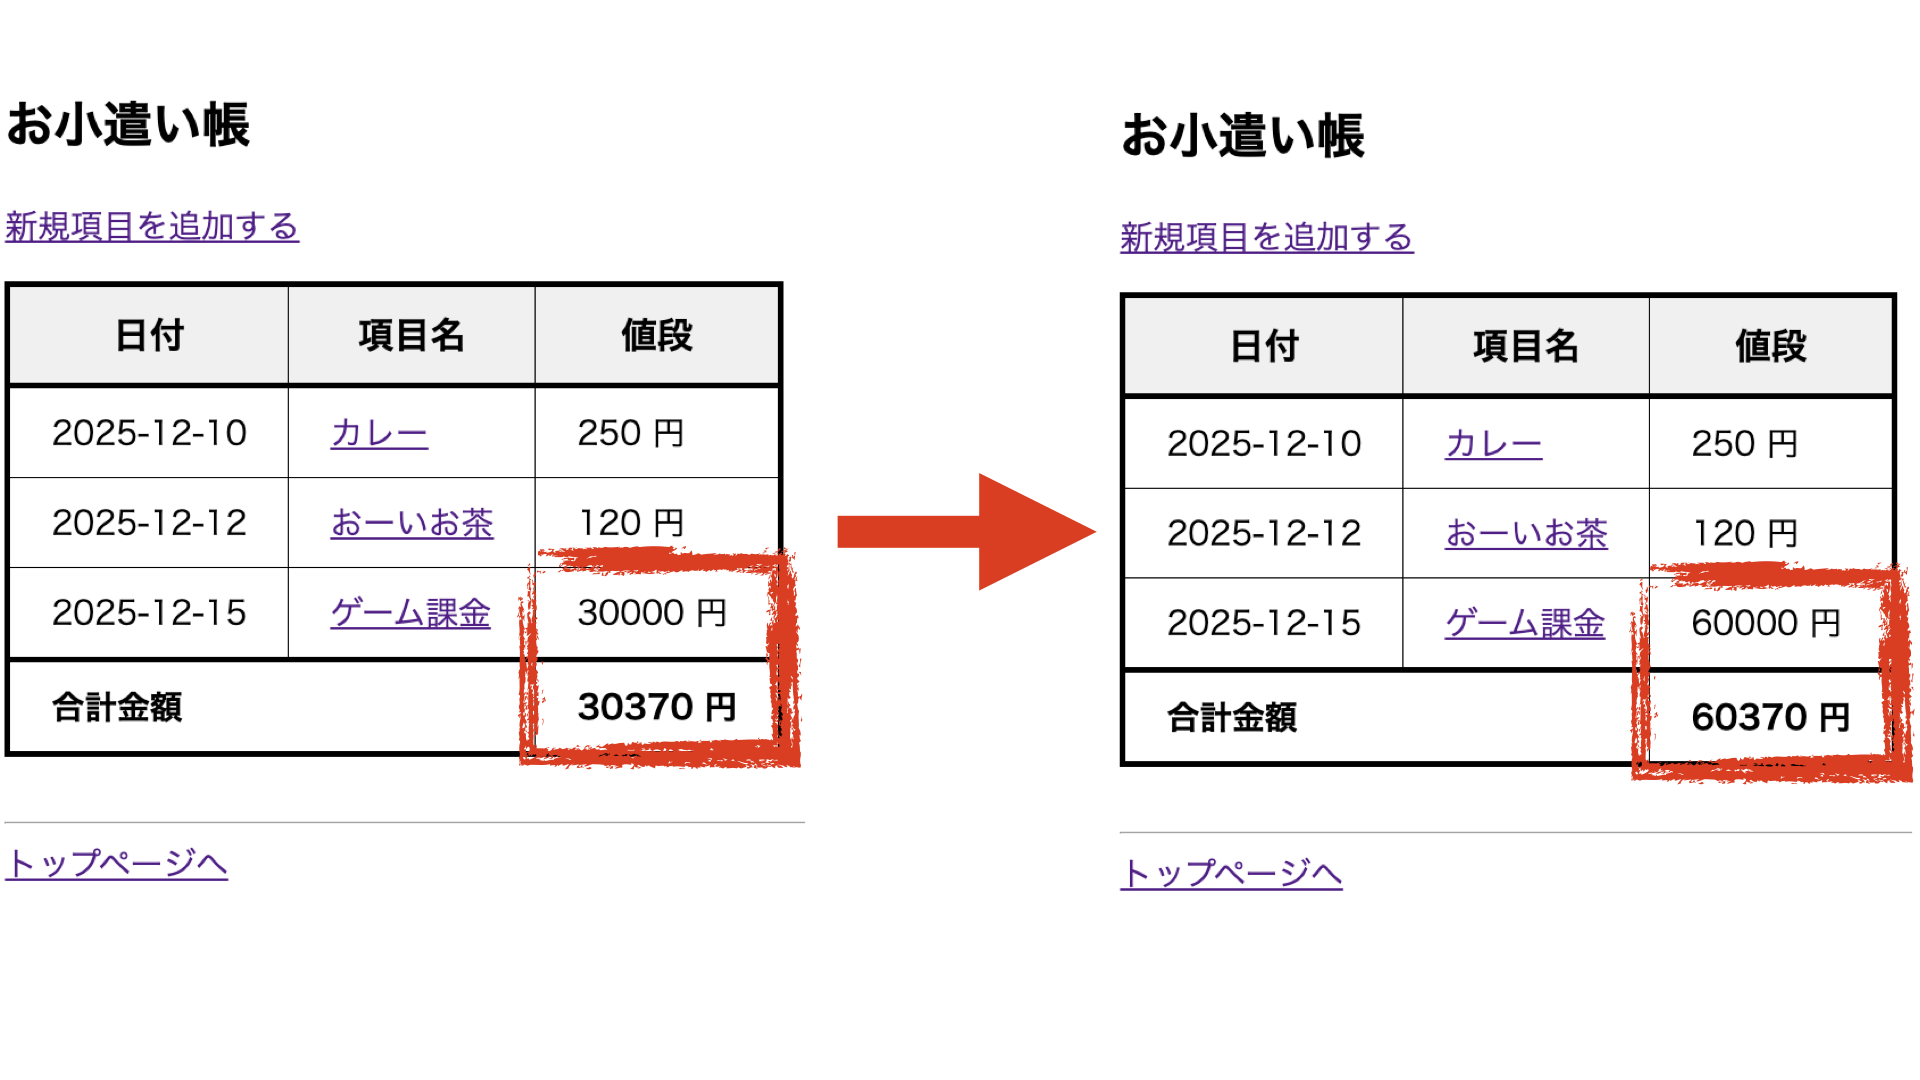
\includegraphics[width=15cm]{fig_web/wallet_edit_fin2.png}
        \caption{編集前と後の一覧表示画面}
        \label{fig:edit_fin2}
        \end{center}
        \end{figure}
\end{enumerate}

\subsection{データの追加}
新しいデータを登録する手順は以下の通りである．
\begin{enumerate}
    \item 一覧表示画面の上方にある「新規項目を追加する」リンクをクリックする（図\ref{fig:go_to_add}）．
        \begin{figure}[H]
        \begin{center}
        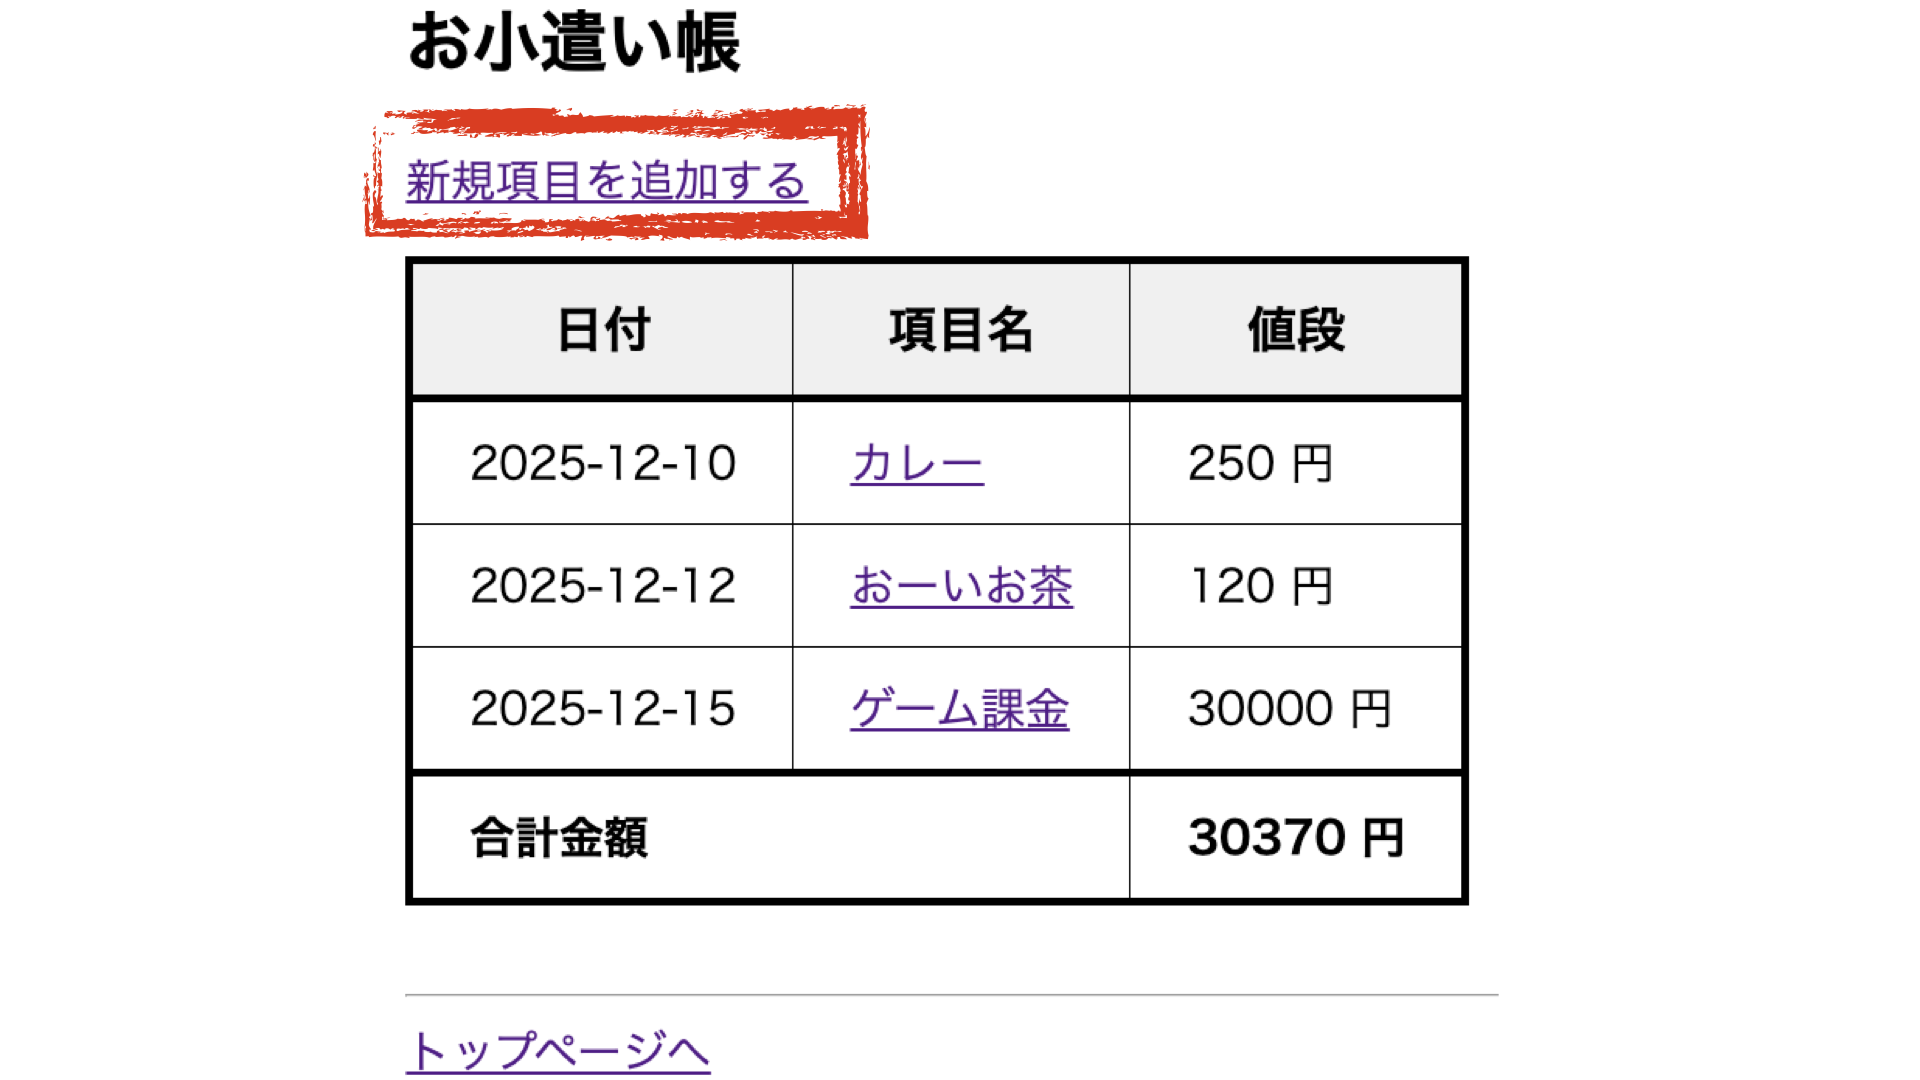
\includegraphics[width=15cm]{fig_web/wallet_go_to_add.png}
        \caption{新規登録画面への行き方}
        \label{fig:go_to_add}
        \end{center}
        \end{figure}
    \item 新規登録画面が表示される（図\ref{fig:add}）．日付，項目名，値段（半角数字），購入目的，備考欄を入力する．
        \begin{figure}[H]
        \begin{center}
        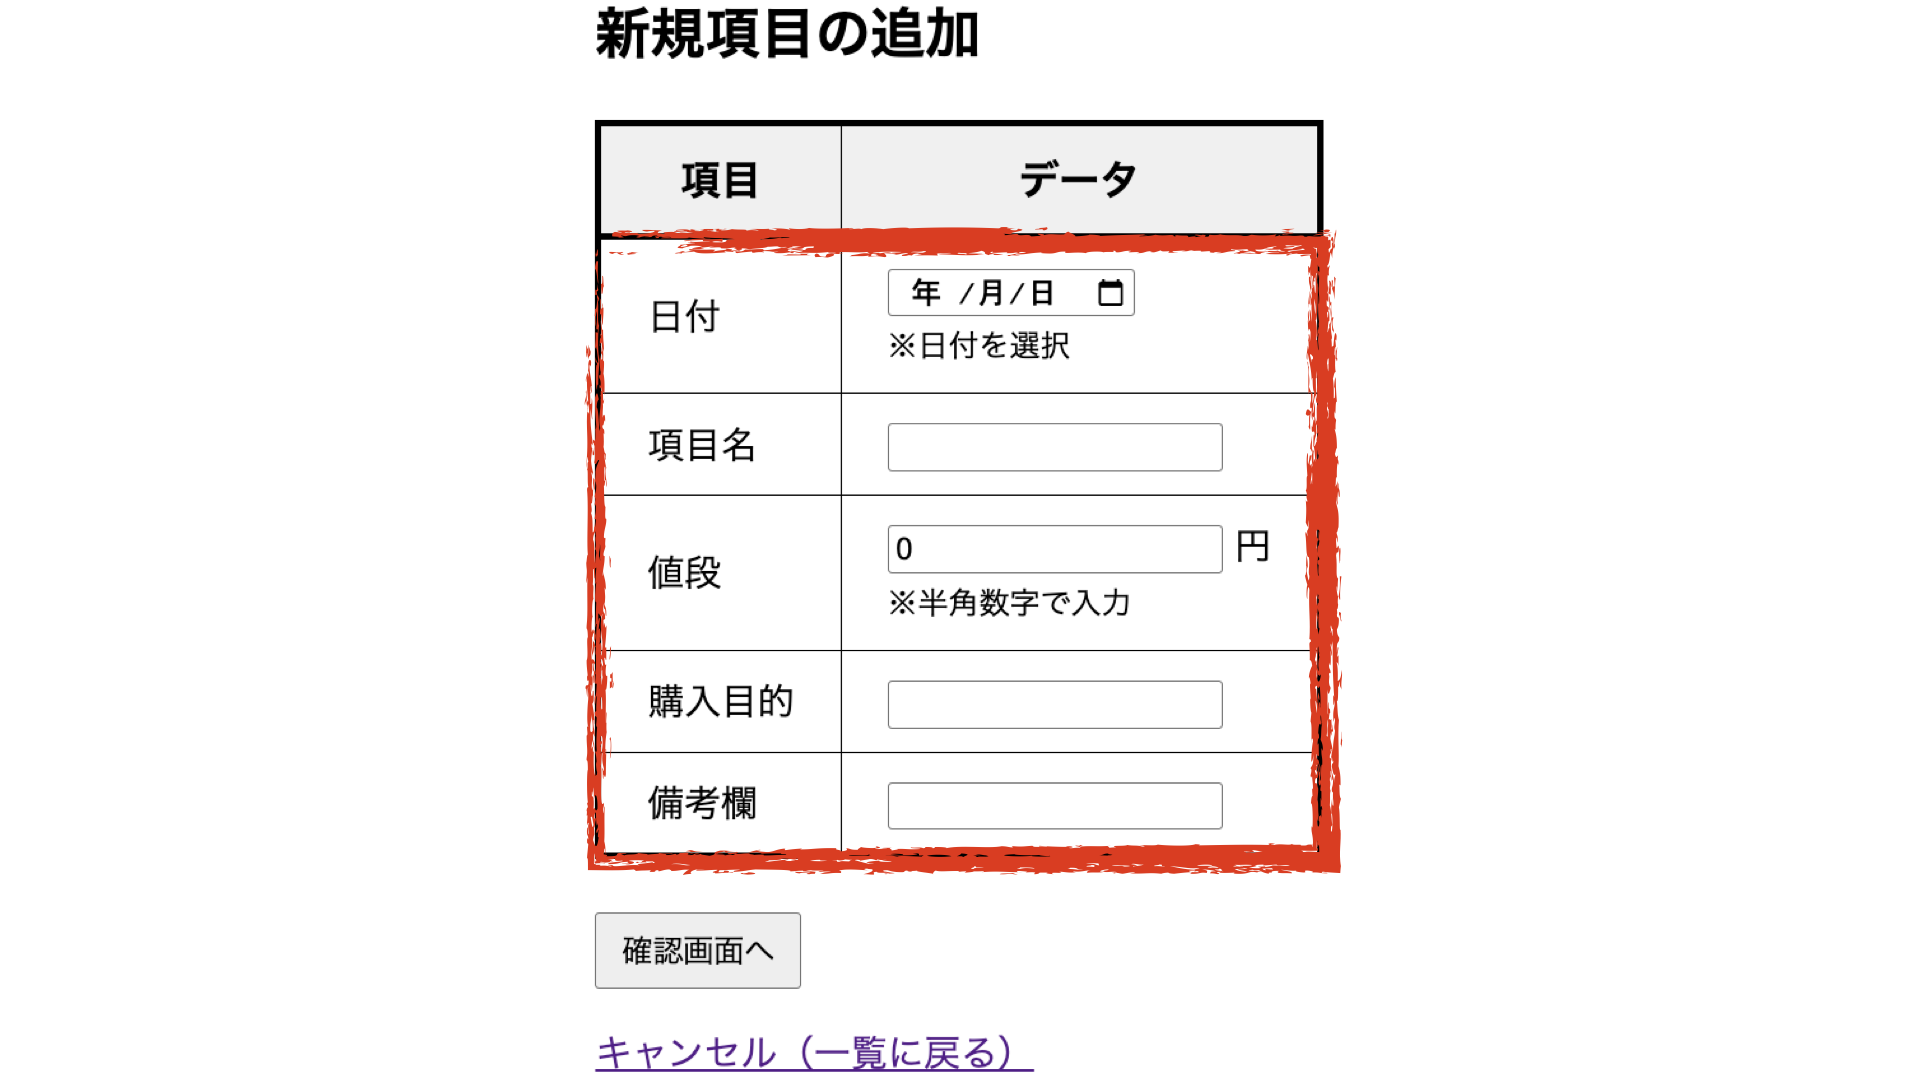
\includegraphics[width=15cm]{fig_web/wallet_add.png}
        \caption{新規登録画面}
        \label{fig:add}
        \end{center}
        \end{figure}
    \item 入力が完了したら「確認画面へ」ボタンを押す（図\ref{fig:add_change}）．
        \begin{figure}[H]
        \begin{center}
        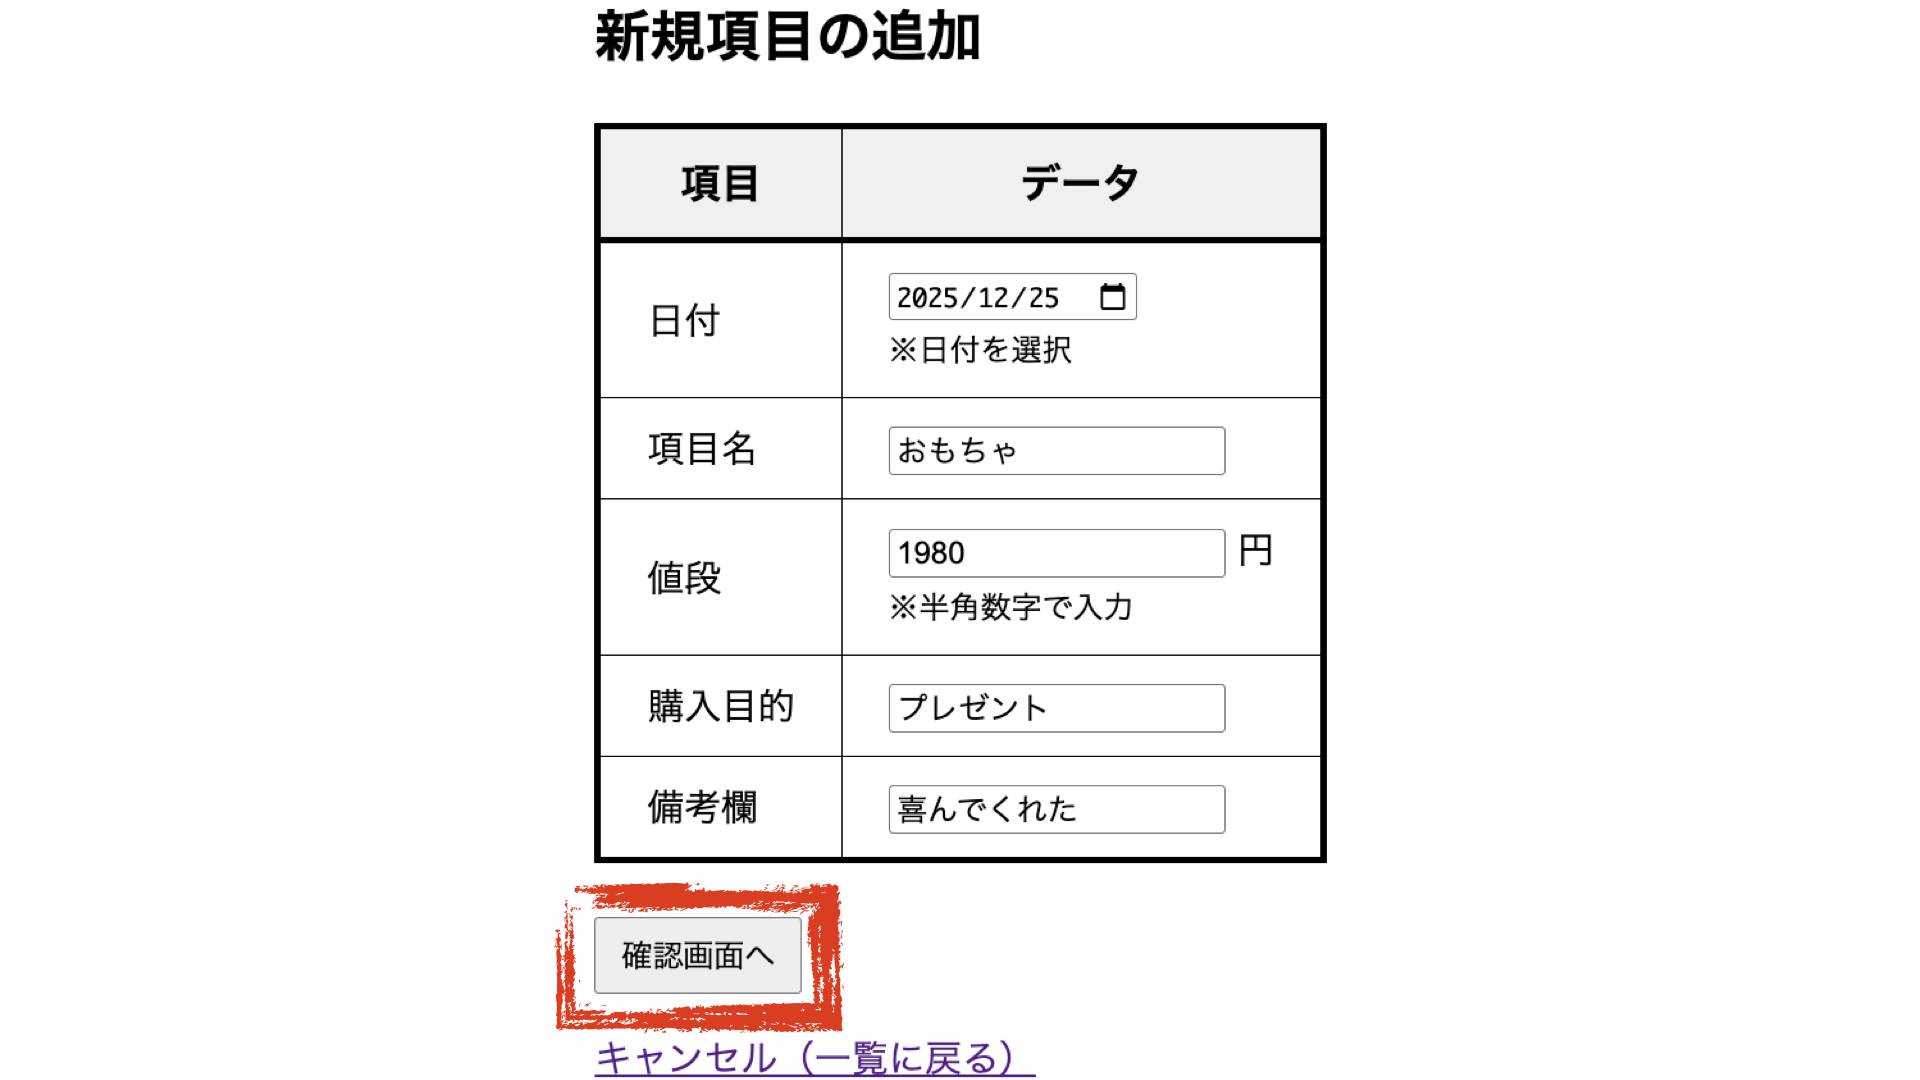
\includegraphics[width=15cm]{fig_web/wallet_add_change.png}
        \caption{新規登録入力例と「確認画面へ」ボタン}
        \label{fig:add_change}
        \end{center}
        \end{figure}
    \item 新規登録内容の確認画面が表示される（図\ref{fig:add_confirm}）．内容に間違いがなければ「追加する」ボタンを押す．修正が必要な場合は「修正する」ボタンを押して入力画面へ戻る．
        \begin{figure}[H]
        \begin{center}
        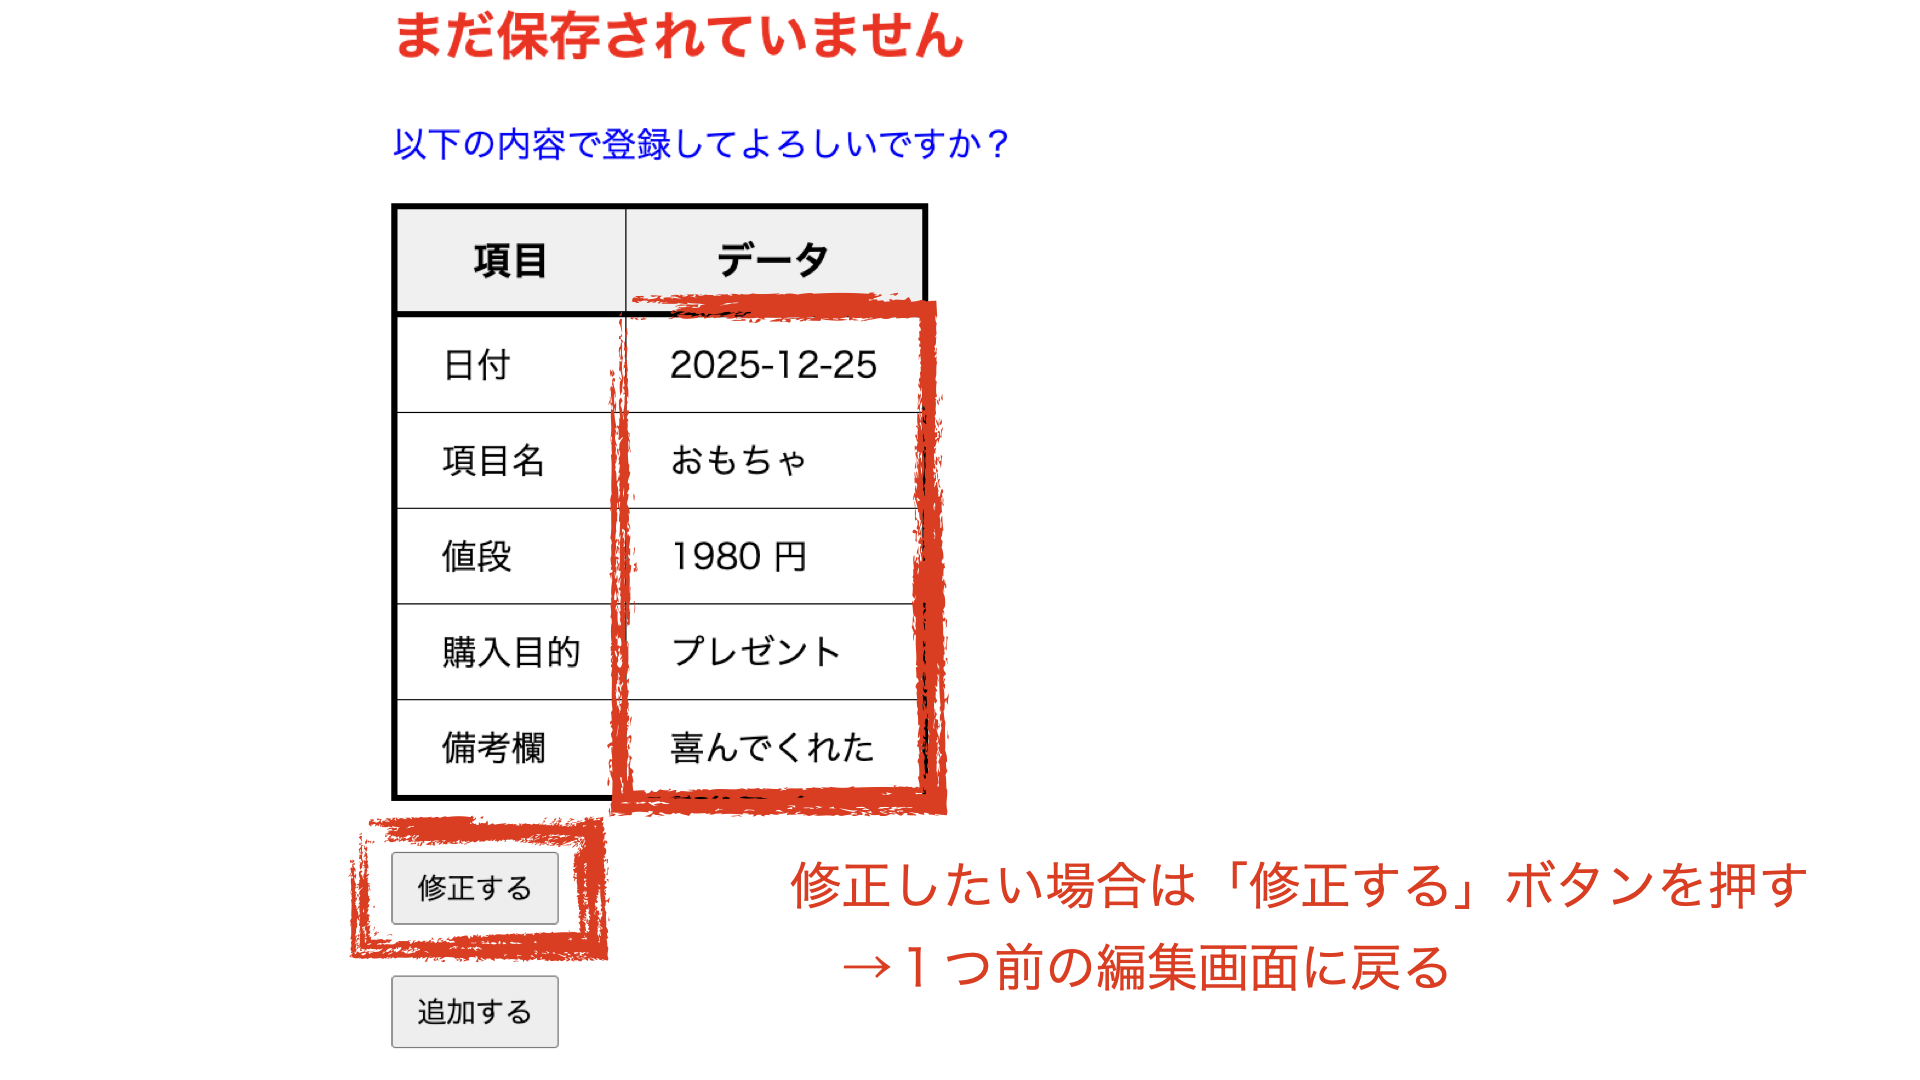
\includegraphics[width=15cm]{fig_web/wallet_add_confirm.png}
        \caption{新規登録内容確認画面}
        \label{fig:add_confirm}
        \end{center}
        \end{figure}
    \item 「追加する」を押すとデータが保存され，一覧表示画面に追加されたデータが表示される（図\ref{fig:add_fin1}）．
        \begin{figure}[H]
        \begin{center}
        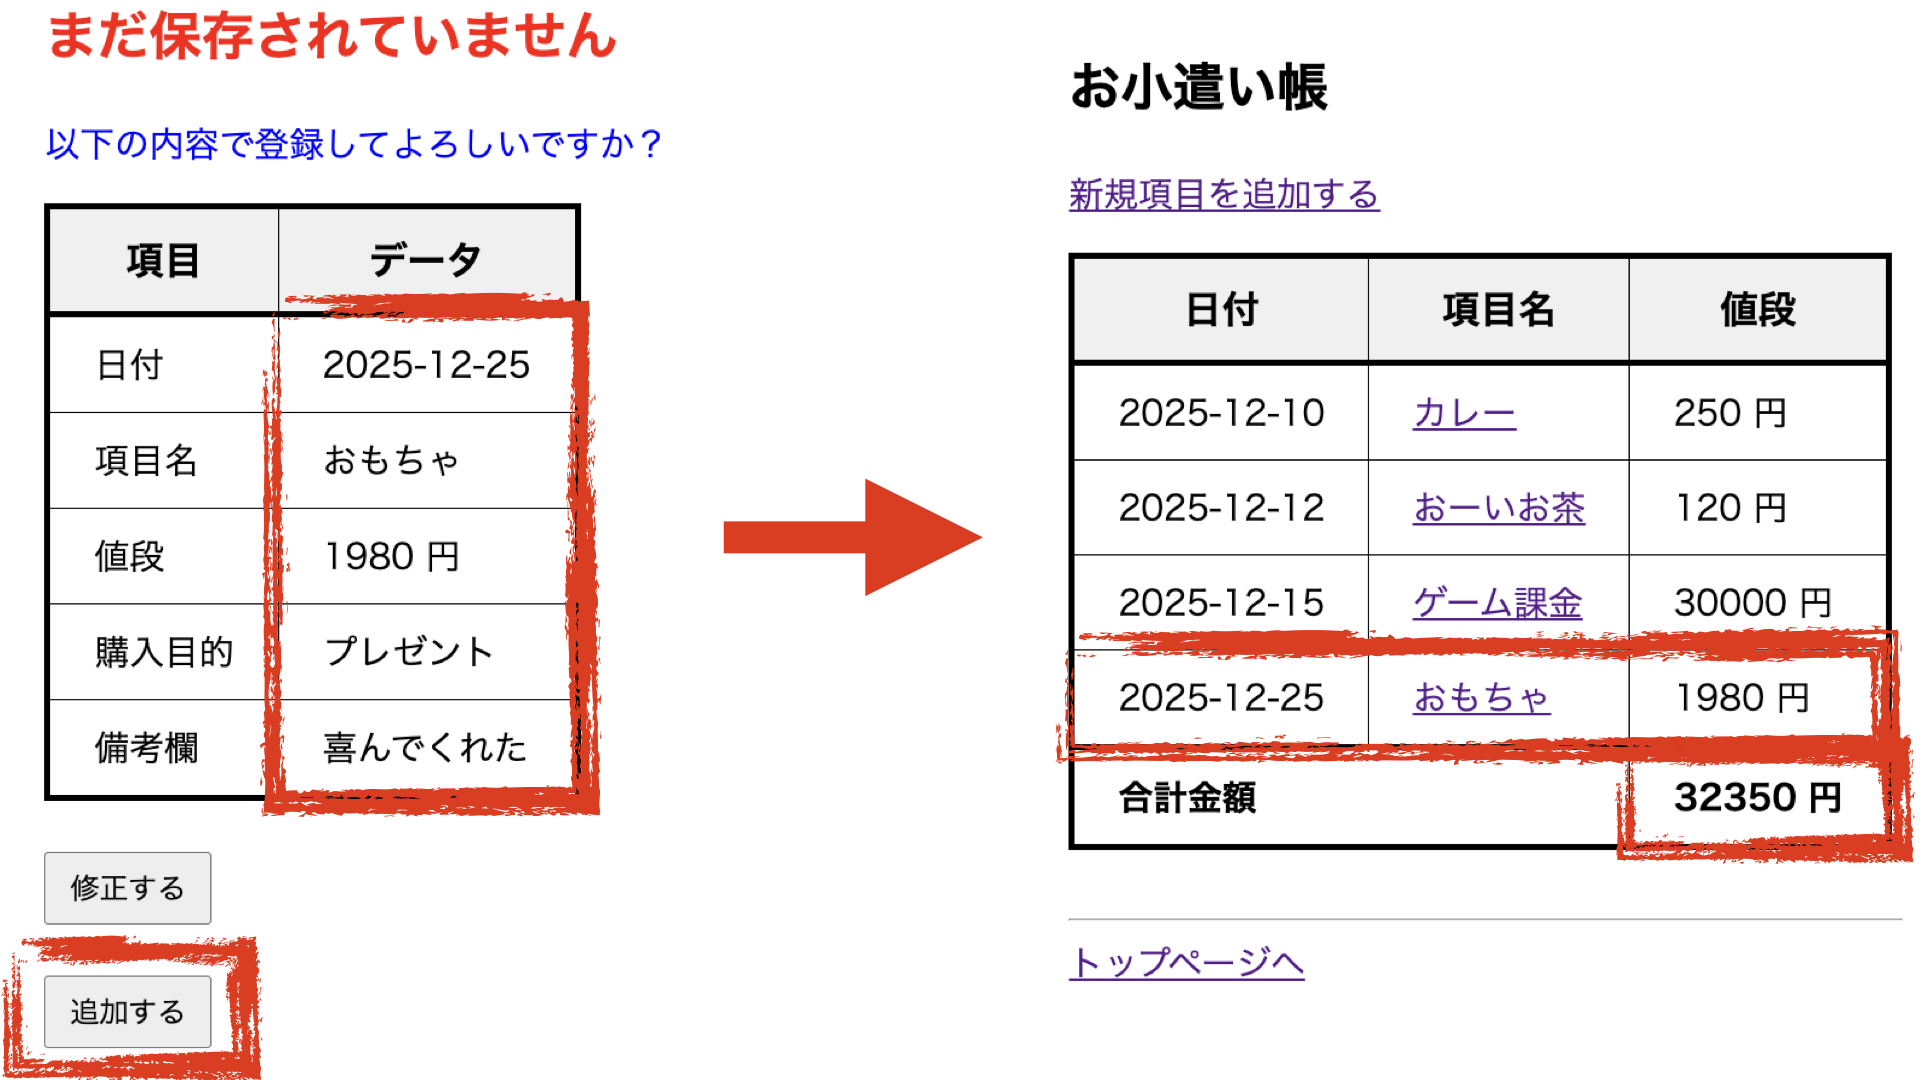
\includegraphics[width=15cm]{fig_web/wallet_add_fin.png}
        \caption{新規登録完了後の画面}
        \label{fig:add_fin1}
        \end{center}
        \end{figure}
\end{enumerate}

\subsection{データの削除}
不要になったデータを削除する手順は以下の通りである．
\begin{enumerate}
    \item 削除したいデータの詳細画面を開き，赤字で表示された「削除する」リンクをクリックする（図\ref{fig:go_to_delete}）．
        \begin{figure}[H]
        \begin{center}
        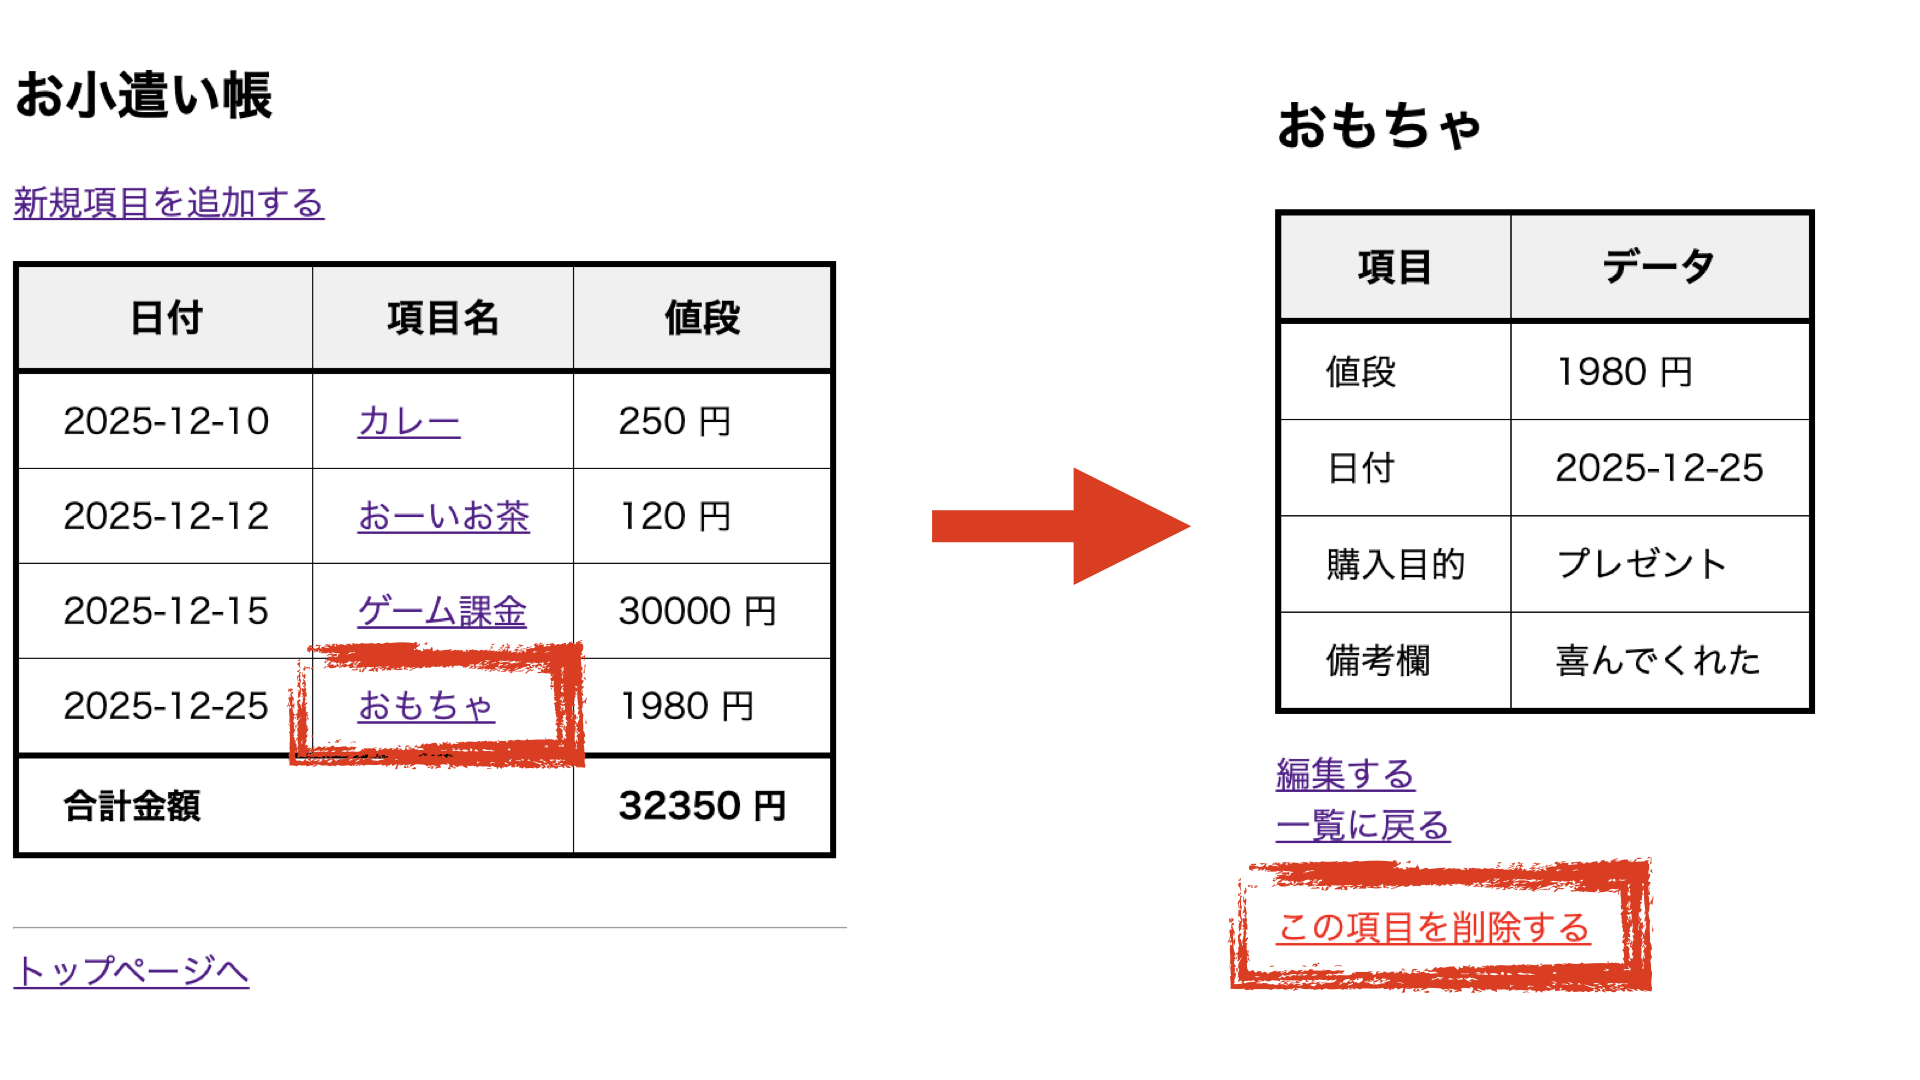
\includegraphics[width=15cm]{fig_web/wallet_go_to_delete.png}
        \caption{削除画面への行き方}
        \label{fig:go_to_delete}
        \end{center}
        \end{figure}
    \clearpage
    \item 削除確認画面が表示される（図\ref{fig:delete_confirm}）．\textbf{この操作は取り消せないため，内容をよく確認する}．削除しない場合は「キャンセル（詳細に戻る）」リンクをクリックする．
        \begin{figure}[H]
        \begin{center}
        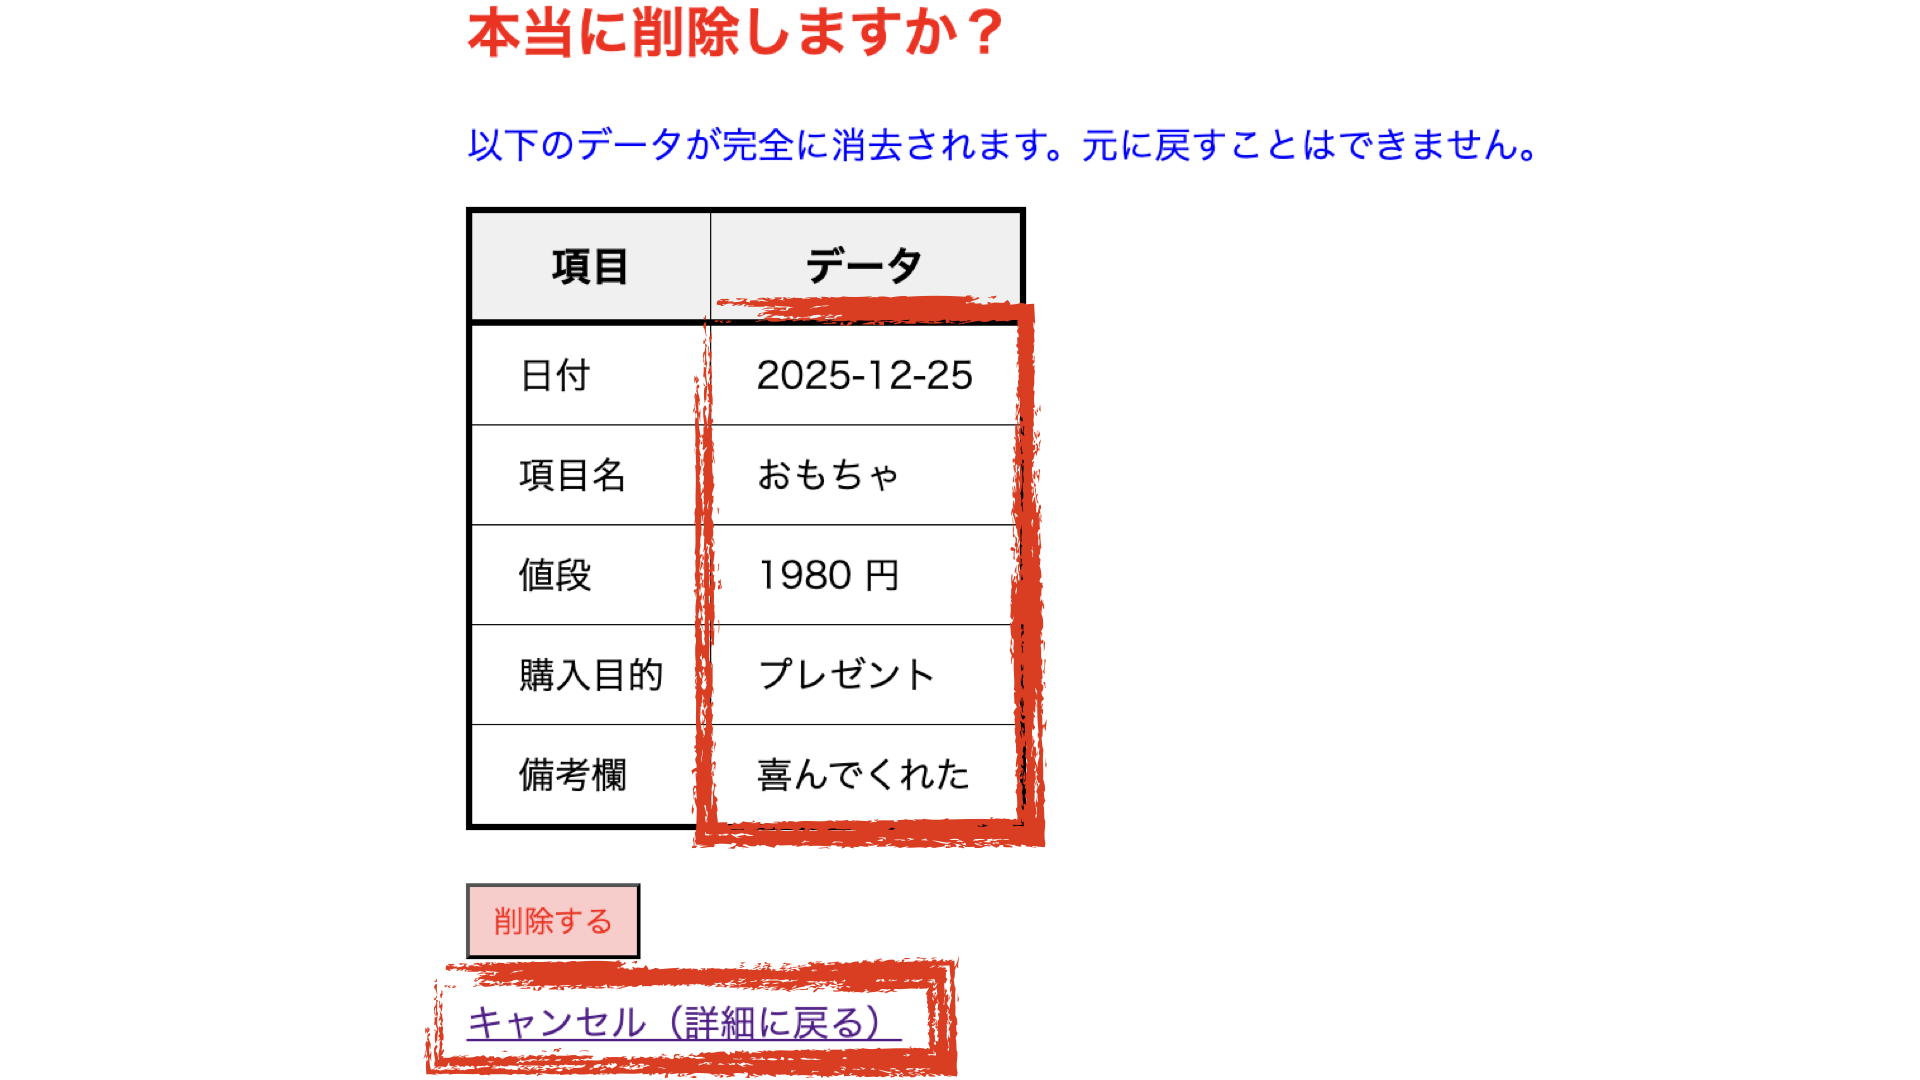
\includegraphics[width=15cm]{fig_web/wallet_delete_confirm.png}
        \caption{削除画面}
        \label{fig:delete_confirm}
        \end{center}
        \end{figure}
    \item \textbf{本当に削除してよければ}「削除する」ボタンを押す（図\ref{fig:delete}）．
        \begin{figure}[H]
        \begin{center}
        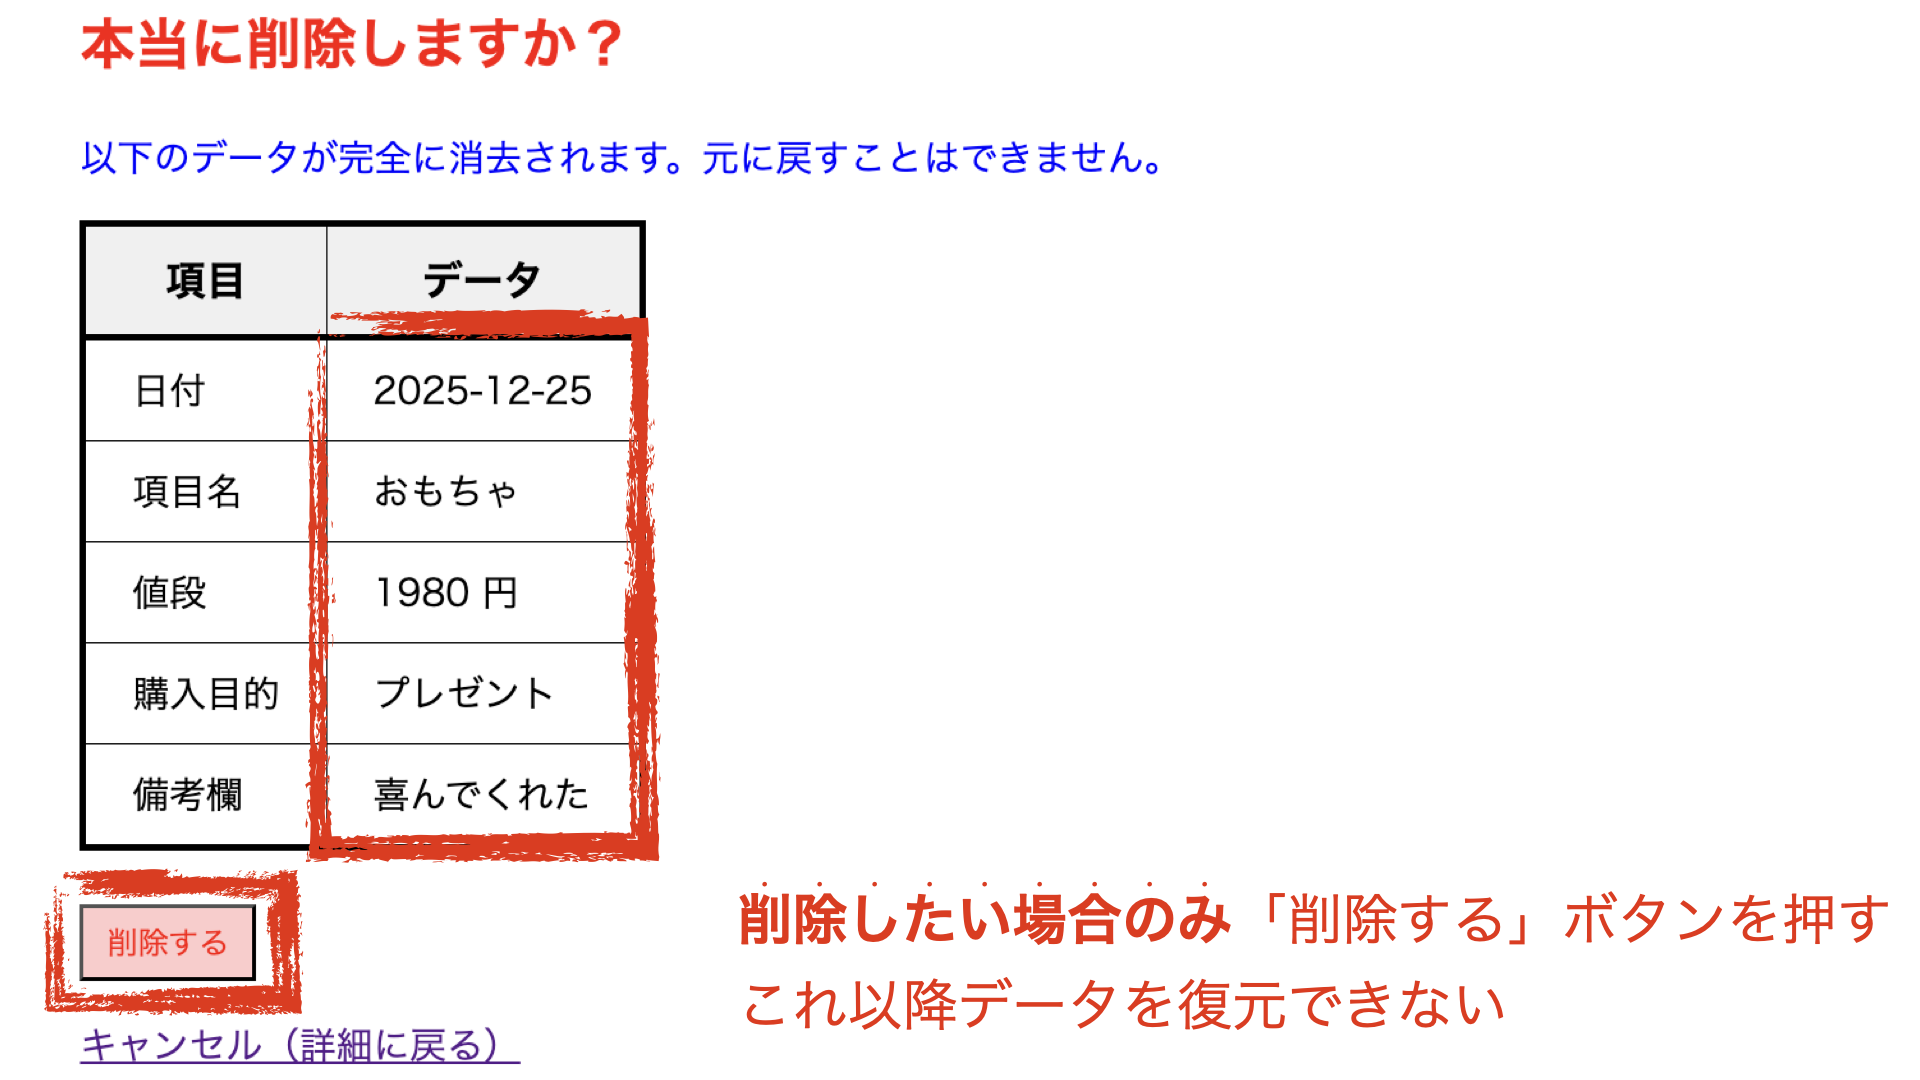
\includegraphics[width=15cm]{fig_web/wallet_delete.png}
        \caption{削除の実行}
        \label{fig:delete}
        \end{center}
        \end{figure}
    \item \textbf{本当に削除してよければ}「OK」を押す（図\ref{fig:delete2}）．これ以降，データの復元ができなくなる．削除をしない場合は「キャンセル」を押す．
        \begin{figure}[H]
        \begin{center}
        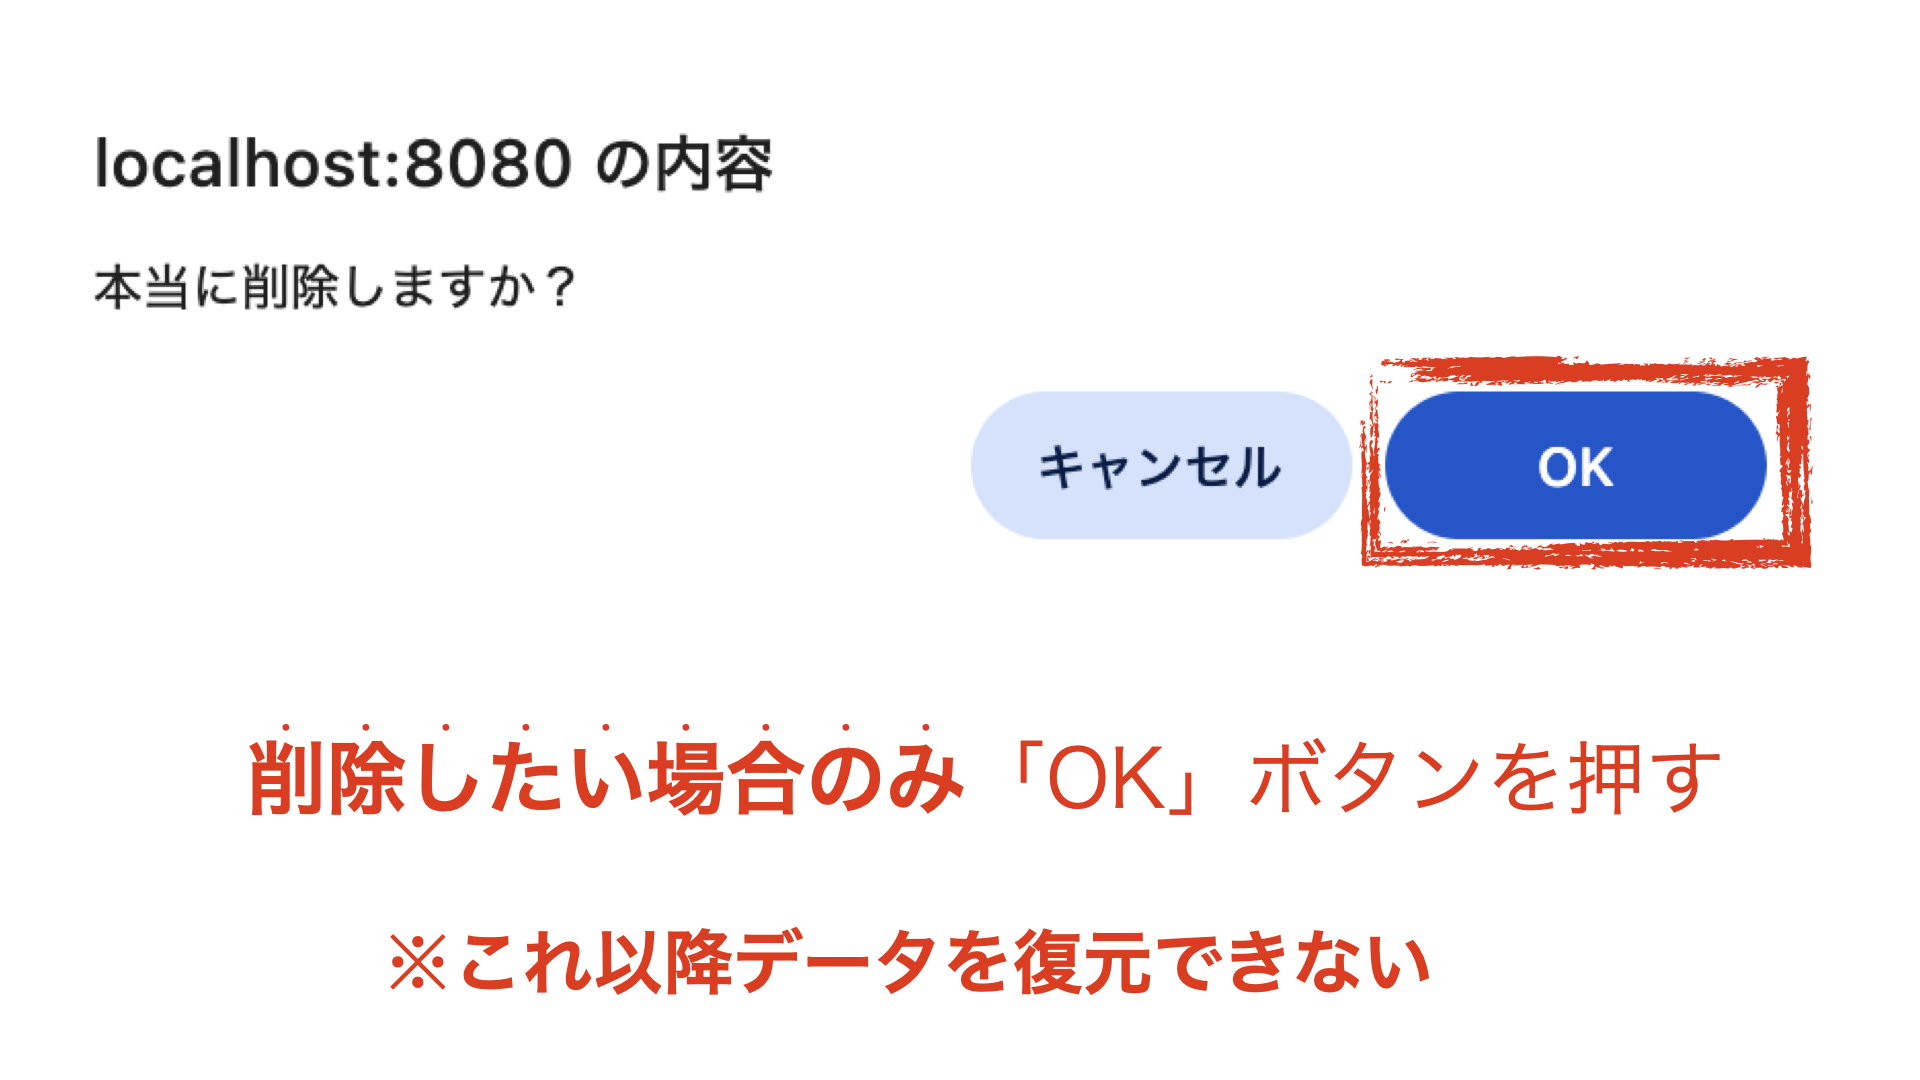
\includegraphics[width=13cm]{fig_web/wallet_delete2.png}
        \caption{削除の最終確認}
        \label{fig:delete2}
        \end{center}
        \end{figure}
    \item データが削除され，一覧画面へ戻る（図\ref{fig:delete_fin}）．一覧表示画面からは削除した項目が無くなっている．
        \begin{figure}[H]
        \begin{center}
        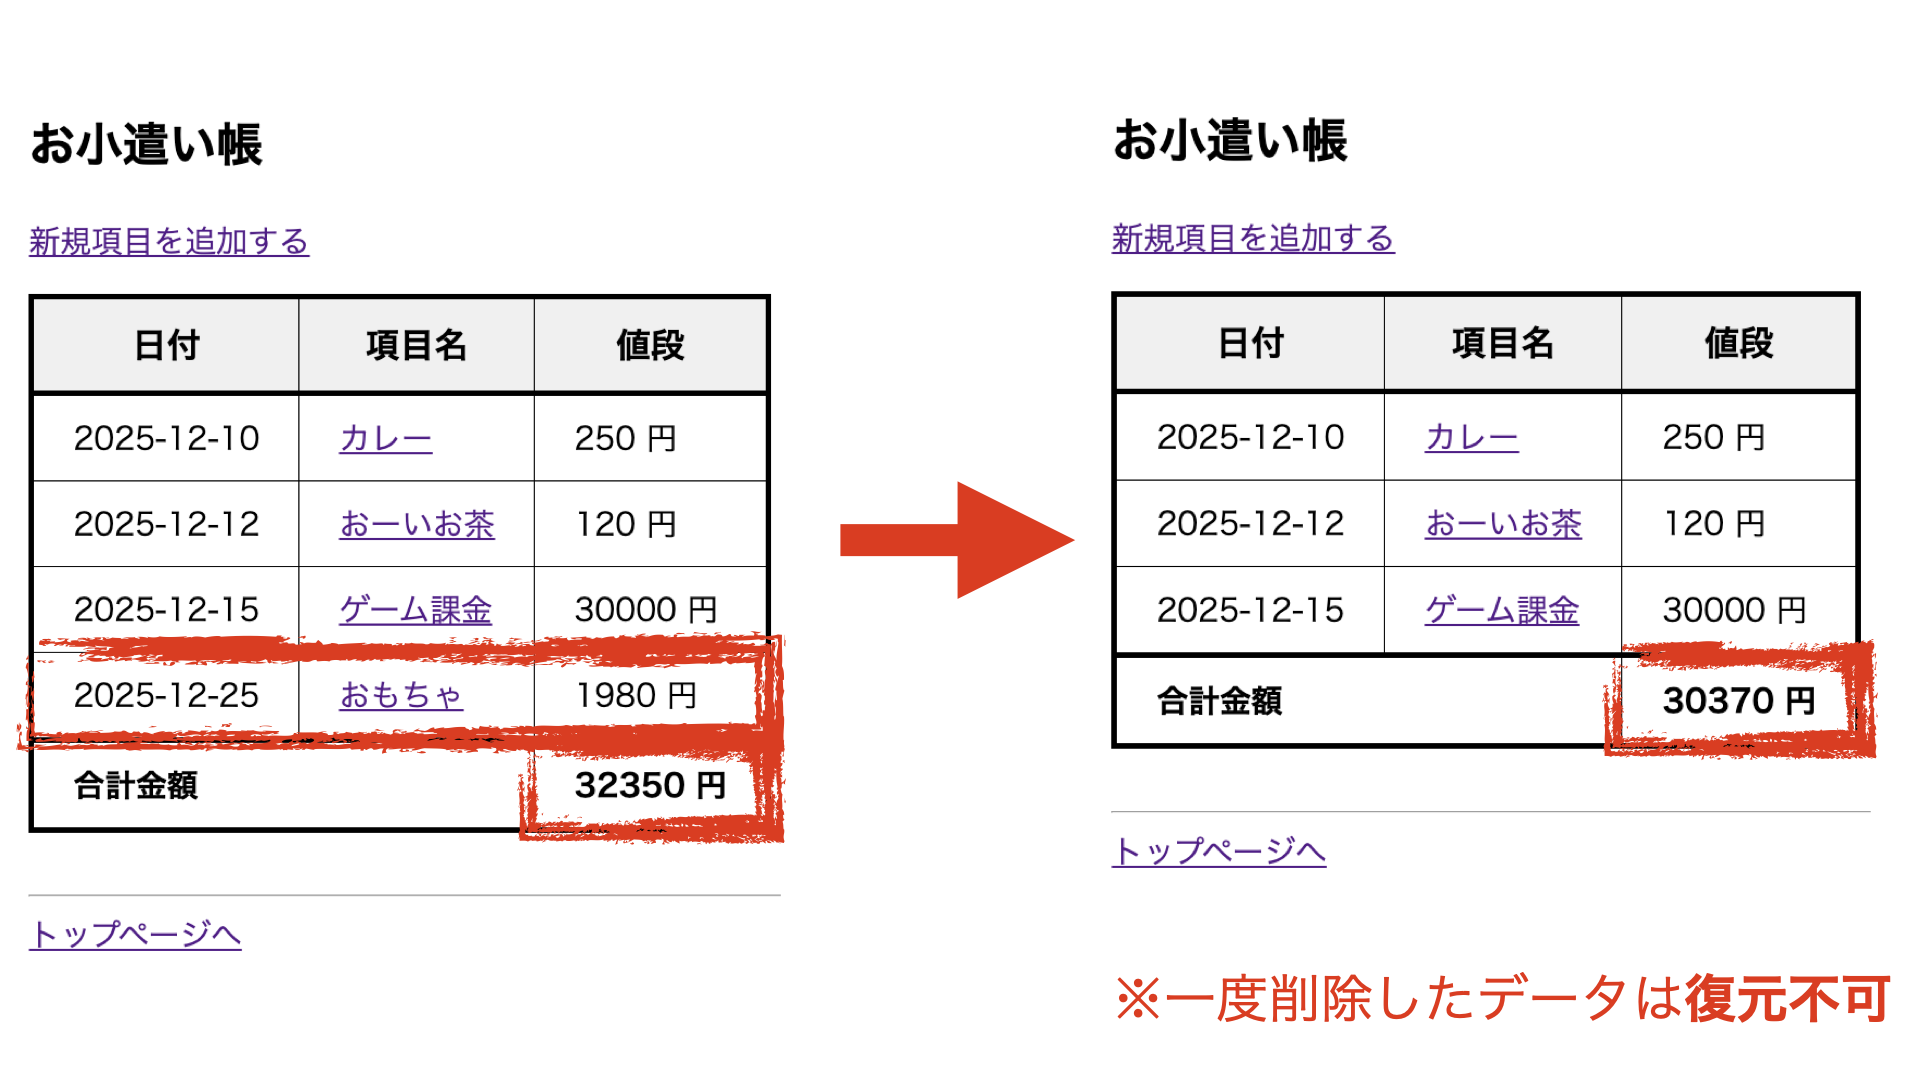
\includegraphics[width=15cm]{fig_web/wallet_delete_fin.png}
        \caption{削除後の一覧表示画面}
        \label{fig:delete_fin}
        \end{center}
        \end{figure}
\end{enumerate}



\section{管理者向けドキュメント}
\subsection{インストール方法}
\subsubsection{システム本体の準備}
本システムのソースコードはGitHubにて公開されている．GitHubのURL（\url{https://github.com/Kuro-aletta/webpro_06}）からリポジトリをダウンロード，またはターミナル上でソースコード\ref{cmd:clone}を実行し，任意のディレクトリに配置する．
\begin{lstlisting}[caption=システム本体のクローン, label=cmd:clone]
$ git clone https://github.com/Kuro-aletta/webpro_06.git
\end{lstlisting}

\subsubsection{ライブラリのインストール}
本システムはNode.js上で動作し，ExpressおよびEJSパッケージを使用する．
ターミナルを開き，システムを配置したディレクトリへ移動した後，ソースコード\ref{cmd:install}のコマンドを実行して必要なライブラリをインストールする．

\begin{lstlisting}[caption=ライブラリのインストール, label=cmd:install]
$ npm install
\end{lstlisting}
これにより，\texttt{package.json} に記載されている，本システムの実行に必要なライブラリ（express, ejs）がまとめてインストールされる．

\subsection{起動方法}
ディレクトリ内に \texttt{app\_report.js} および \texttt{node\_modules} フォルダが存在することを確認する．
確認後，ソースコード\ref{cmd:start}のコマンドを実行してサーバを起動する．
\begin{lstlisting}[caption=システムの起動, label=cmd:start]
$ node app_report.js
\end{lstlisting}
「Example app listening on port 8080!」と表示されれば起動成功である．
Webブラウザで以下のURLにアクセスして動作を確認する．
\begin{itemize}
    \item トップページ: \url{http://localhost:8080/}
    \item 成績管理システム: \url{http://localhost:8080/result}
    \item 教員情報システム: \url{http://localhost:8080/teacher}
    \item お小遣い帳システム: \url{http://localhost:8080/wallet}
\end{itemize}

\subsection{起動できない場合}
\subsubsection{ライブラリが見つからない場合}
起動時に \texttt{Error: Cannot find module 'express'} と表示される場合は，ライブラリのインストールが行われていない．\texttt{npm install} コマンド（ソースコード\ref{cmd:install}）を再度実行することで解決する．

\subsubsection{ポート番号が既に使用されている場合}
起動時に \texttt{Error: listen EADDRINUSE: address already in use :::8080} と表示される場合は，既に別のプロセスが8080番ポートを使用している．
これは多くの場合，前回のサーバ起動時に正しく終了できず，バックグラウンドでプロセスが動作し続けていることに起因する．
この場合，以下の手順でプロセスを特定し，停止させる必要がある．

\begin{enumerate}
    \item ポート8080を使用しているプロセスのID（PID）を特定する（ソースコード\ref{cmd:lsof}）．
\begin{lstlisting}[caption=PIDの確認, label=cmd:lsof]
$ lsof -i :8080
\end{lstlisting}
    \item 表示されたPID（数値）を指定してプロセスを終了（kill）する（ソースコード\ref{cmd:kill}）．
\begin{lstlisting}[caption=プロセスの終了, label=cmd:kill]
$ kill <PID>
\end{lstlisting}
    \item 上記コマンド（ソースコード\ref{cmd:kill}）でも終了しない（強制終了が必要な）場合は，\texttt{-9} を付けて再度実行する（ソースコード\ref{cmd:kill9}）．
\begin{lstlisting}[caption=プロセスの強制終了, label=cmd:kill9]
$ kill -9 <PID>
\end{lstlisting}
\end{enumerate}

なお，\texttt{app\_report.js} 内のポート番号設定（\texttt{app.listen(8080, ...)} の部分）を別の番号（8081など）に書き換えることでも対応可能であるが，アクセスするURLが変更となり利用者への周知が必要となるため，この方法は推奨しない．

\subsection{終了方法}
サーバを停止させる場合は，起動しているターミナル上で \texttt{Ctrl + C} キーを入力する．
なお，\texttt{Ctrl + Z} はプロセスを一時停止させる操作であり，完全に終了しない．この状態でターミナルを閉じるとポートが占有されたままとなり，次回の起動時にエラー（EADDRINUSE）の原因となるため注意が必要である．

\subsection{分かっている不具合・制限事項}
本システムはデータをサーバのメモリ上に保存しているため，サーバを再起動または終了すると，登録したデータはすべてリセットされる仕様である．
なお，現在確認されている動作上の不具合はない．




\section{開発者向けドキュメント}
\subsection{概要}
本システムは，サーバサイドJavaScript実行環境であるNode.jsおよびWebフレームワークExpressを用いて構築されたWebアプリケーションである．
アーキテクチャとしてMVC（Model-View-Controller）モデルに近い構成を採用しており，\texttt{views} ディレクトリ内のEJSテンプレート（View）と，\texttt{app\_report.js} によるルーティングおよびロジック処理（Controller）により動作する．
なお，本システムではデータベースを使用せず，サーバメモリ上の変数（配列）としてデータを管理する（Model相当）仕様としている．

\subsection{開発環境}
本システムの開発および動作環境は以下の通りである．
\begin{itemize}
    \item 実行環境: Node.js (v24.3.0)
    \item 言語: JavaScript
    \item フレームワーク: Express
    \item テンプレートエンジン: EJS
\end{itemize}

\subsection{ディレクトリ構造}
GitHub（\url{https://github.com/Kuro-aletta/webpro_06}）にて公開されている本システムのファイル構成を図\ref{fig:dir_tree}に示す．なお，本システムに関与しないファイルは省略されている．
実行の起点となるプログラムである \texttt{app\_report.js} をルートに置き，静的リソース（CSSなど）は \texttt{public} ディレクトリ，画面のひな型となるEJSファイルは \texttt{views} ディレクトリに配置して管理している．

\begin{figure}[H]
\renewcommand*\DTstylecomment{\rmfamily\color{black}\footnotesize\itshape} % コメントのスタイル調整（任意）
\dirtree{%
.1 webpro\_06/.
.2 app\_report.js \DTcomment{サーバサイドプログラム}.
.2 package.json \DTcomment{依存ライブラリ定義}.
.2 node\_modules/ \DTcomment{インストールされたライブラリ}.
.2 public/ \DTcomment{静的ファイル用ディレクトリ}.
.3 style.css \DTcomment{共通スタイルシート}.
.3 top.html \DTcomment{トップページ}.
.2 views/ \DTcomment{EJSファイル用ディレクトリ}.
.3 result\_list.ejs \DTcomment{成績:一覧}.
.3 result\_detail.ejs \DTcomment{成績:詳細}.
.3 result\_add.ejs \DTcomment{成績:追加入力}.
.3 result\_add\_confirm.ejs \DTcomment{成績:追加確認}.
.3 result\_edit.ejs \DTcomment{成績:編集入力}.
.3 result\_edit\_confirm.ejs \DTcomment{成績:編集確認}.
.3 result\_delete\_confirm.ejs \DTcomment{成績:削除確認}.
.3 teacher\_list.ejs \DTcomment{教員:一覧}.
.3 teacher\_detail.ejs \DTcomment{教員:詳細}.
.3 teacher\_add.ejs \DTcomment{教員:追加入力}.
.3 teacher\_add\_confirm.ejs \DTcomment{教員:追加確認}.
.3 teacher\_edit.ejs \DTcomment{教員:編集入力}.
.3 teacher\_edit\_confirm.ejs \DTcomment{教員:編集確認}.
.3 teacher\_delete\_confirm.ejs \DTcomment{教員:削除確認}.
.3 wallet\_list.ejs \DTcomment{財布:一覧}.
.3 wallet\_detail.ejs \DTcomment{財布:詳細}.
.3 wallet\_add.ejs \DTcomment{財布:追加入力}.
.3 wallet\_add\_confirm.ejs \DTcomment{財布:追加確認}.
.3 wallet\_edit.ejs \DTcomment{財布:編集入力}.
.3 wallet\_edit\_confirm.ejs \DTcomment{財布:編集確認}.
.3 wallet\_delete\_confirm.ejs \DTcomment{財布:削除確認}.
}
\caption{ディレクトリ構造}
\label{fig:dir_tree}
\end{figure}

\subsection{システム構造とURL設計}
本システムは，\texttt{app\_report.js} を実行し，\texttt{views/} ディレクトリ内のEJSファイルをもとにHTMLを生成して表示する構成をとっている．
データの永続化は行わず，サーバメモリ上の変数（配列）としてデータを保持する仕様とした．

各システムにおけるページ遷移図を図\ref{fig:md}に，HTTPメソッド，リソース名（URL）の対応を表\ref{tab:url}に示す．
\begin{figure}[H]
 \begin{center}
  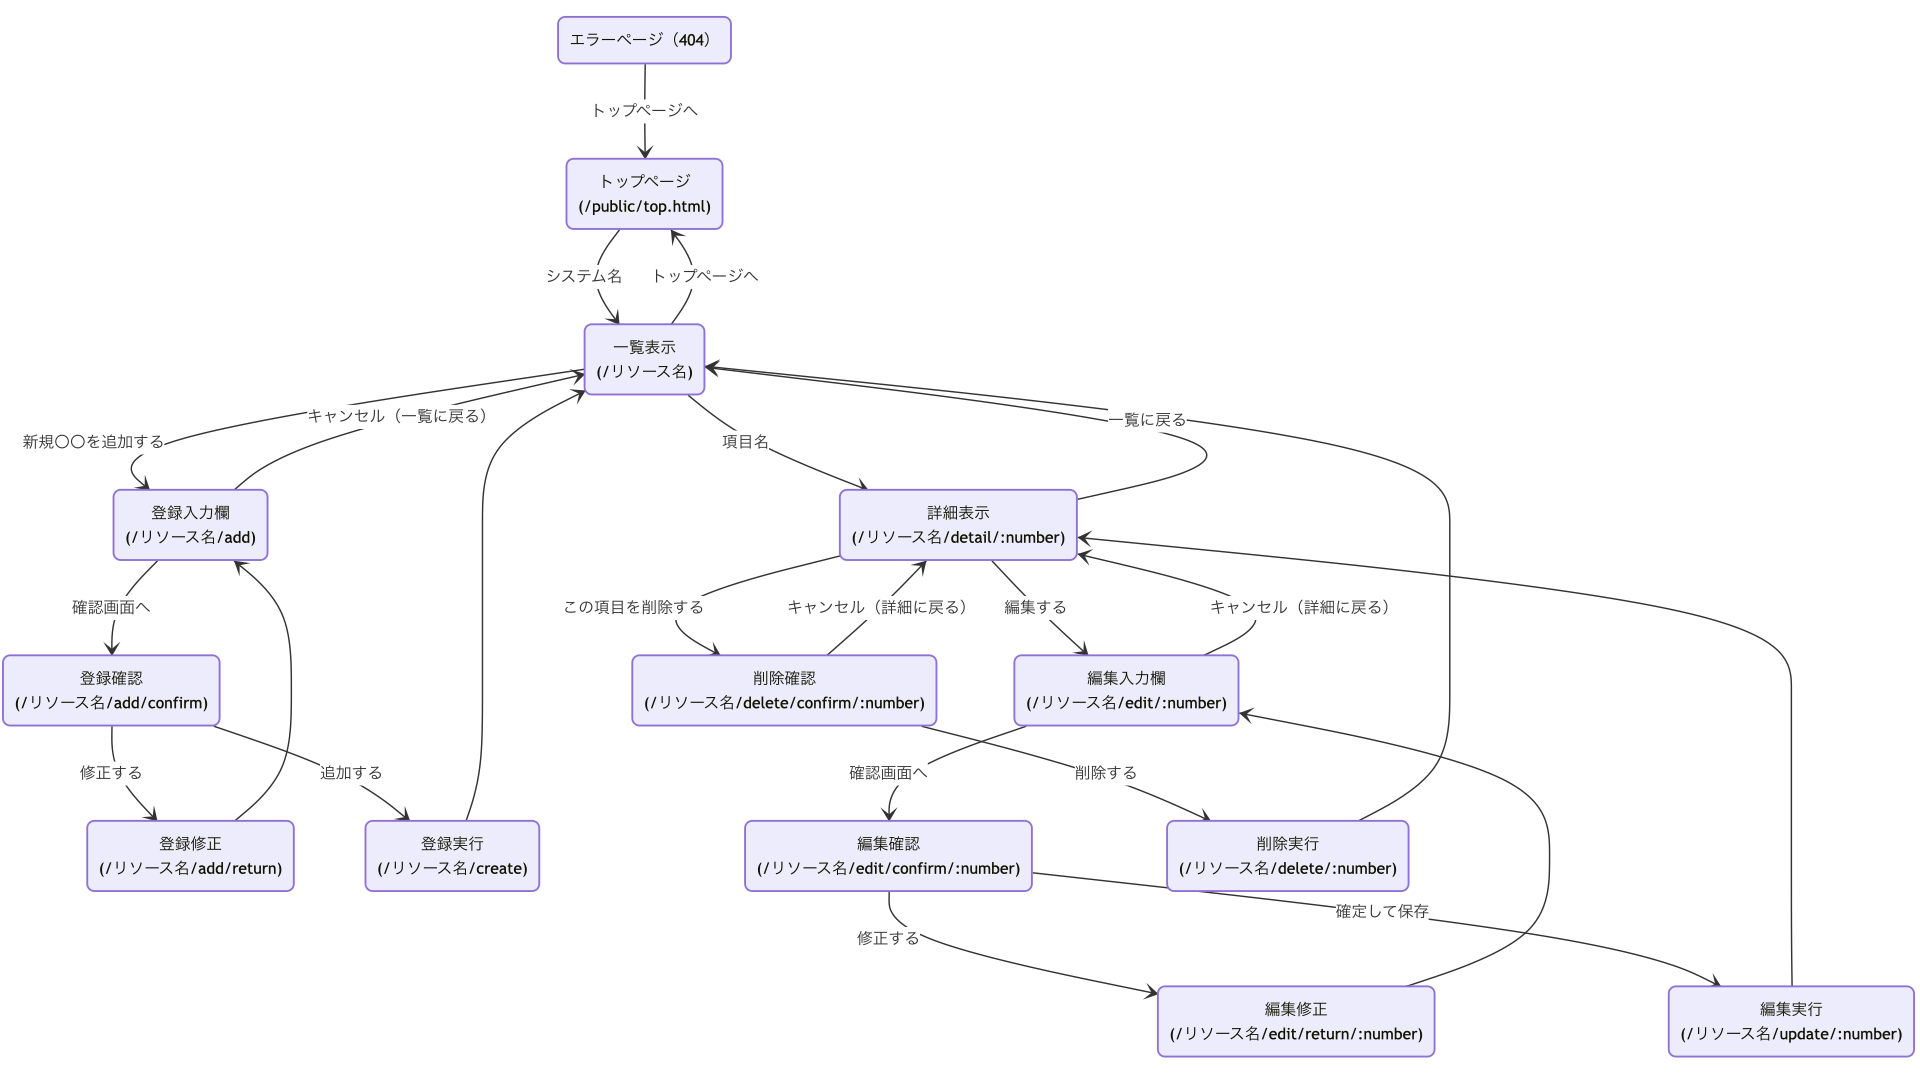
\includegraphics[width=1\linewidth]{fig_web/md.png}
  \caption{ページ遷移図}
  \label{fig:md}
 \end{center}
\end{figure}
\begin{table}[H]
\caption{URL設計とHTTPメソッド}
\label{tab:url}
\centering
\begin{tabular}{l|l|l}
\hline
画面・機能 & HTTPメソッド & URLパターン \\
\hline \hline
トップページ & GET & \texttt{/} \\
\hline
一覧表示 & GET & \texttt{/リソース名} \\
詳細表示 & GET & \texttt{/リソース名/detail/:number} \\
新規登録（入力） & GET & \texttt{/リソース名/add} \\
新規登録（確認） & POST & \texttt{/リソース名/add/confirm} \\
新規登録（修正） & POST & \texttt{/リソース名/add/return} \\
新規登録（実行） & POST & \texttt{/リソース名/create} \\
編集（入力） & GET & \texttt{/リソース名/edit/:number} \\
編集（確認） & POST & \texttt{/リソース名/edit/confirm/:number} \\
編集（修正） & POST & \texttt{/リソース名/edit/return/:number} \\
編集（実行） & POST & \texttt{/リソース名/update/:number} \\
削除（確認） & GET & \texttt{/リソース名/delete/confirm/:number} \\
削除（実行） & POST & \texttt{/リソース名/delete/:number} \\
\hline
エラー（404） & ALL & - \\
\hline
\end{tabular}
\end{table}
\clearpage
各システムのリソース名は以下の通りである．
\begin{itemize}
    \item 成績管理システム: \texttt{result}
    \item 教員情報システム: \texttt{teacher}
    \item お小遣い帳システム: \texttt{wallet}
\end{itemize}

以下に，本システムの画面遷移やデータの受け渡しに関する詳細な仕組みを述べる．

\subsubsection{ページ遷移の仕組み}
各画面間の遷移は，主に以下の2つの方法で行われる．
\begin{itemize}
    \item \textbf{参照（GET）}: 一覧画面の各項目やメニューのリンク（\texttt{<a>}タグ）をクリックすることで遷移する．
    \item \textbf{操作（POST）}: 登録・編集・削除の確認画面や実行処理へは，フォーム（\texttt{<form>}タグ）の送信ボタンをクリックすることで遷移する．
\end{itemize}

\subsubsection{データの受け渡し（リレー方式）}
新規登録や編集の際，入力画面から確認画面を経て実行処理へと進む過程で，一度サーバに送信したデータを維持する必要がある．
本システムでは，HTTPの直前の状態を保持しない特性を補うため，確認画面のフォーム内に \texttt{type="hidden"} 属性を持つ \texttt{input} タグを配置し，次画面へ再度データを送信して受け渡す「リレー方式」を採用した．

\subsubsection{処理実行後の画面遷移}
データの追加・更新・削除が完了した後の遷移先は，ユーザビリティを考慮して以下のように設計した．
\begin{itemize}
    \item \textbf{追加・削除後}: 作業結果全体を確認しやすくするため，「一覧表示画面」へリダイレクトする．
    \item \textbf{編集後}: 変更内容を即座に確認できるようにするため，そのデータの「詳細表示画面」へリダイレクトする．
\end{itemize}

\clearpage
\subsection{データ構造}
各システムは，オブジェクトの配列としてデータを管理している．それぞれのデータ構造を以下に示す．

\subsubsection{成績管理システム (result)}
履修科目の成績情報を管理する．
\begin{table}[H]
\caption{成績データの構造}
\centering
\begin{tabular}{l|l|l}
\hline
項目名 & 変数名 & 説明 \\
\hline \hline
年度 & year & 開講年度（数値） \\
セメスタ & semester & 開講学期（数値） \\
科目名 & name & 講義の名称 \\
担当教員 & teacher & 教員名 \\
副担当 & subteacher & 副担当教員名（任意） \\
単位数 & credit & 科目の単位数（数値） \\
成績 & grade & S, A, B, C, 合 など \\
\hline
\end{tabular}
\end{table}

\subsubsection{教員情報システム (teacher)}
教員の所属や担当科目などの情報を管理する．
\begin{table}[H]
\caption{教員データの構造}
\centering
\begin{tabular}{l|l|l}
\hline
項目名 & 変数名 & 説明 \\
\hline \hline
学科 & department & 所属学科名 \\
氏名 & name & 教員名 \\
職位 & job & 教授，准教授など \\
研究室 & laboratory & 研究室名 \\
担当科目 & subject & 主な担当科目 \\
\hline
\end{tabular}
\end{table}

\subsubsection{お小遣い帳システム (wallet)}
金銭の出納記録を管理する．合計金額の計算に使用するため，\texttt{price} は必ず数値型として扱う．
\begin{table}[H]
\caption{お小遣い帳データの構造}
\centering
\begin{tabular}{l|l|l}
\hline
項目名 & 変数名 & 説明 \\
\hline \hline
日付 & date & 利用日（YYYY-MM-DD形式） \\
項目名 & item & 購入品目などの名称 \\
値段 & price & 金額（数値） \\
購入目的 & purpose & 利用の目的 \\
備考欄 & memo & メモ \\
\hline
\end{tabular}
\end{table}

\subsection{各システムの機能詳細}
\subsubsection{成績管理システム}
履修データの登録・編集・削除を行う．
一覧画面では，科目名(\texttt{name})をクリックすることで詳細画面へ遷移する．教員名が未入力の場合は「（科目名を設定してください）」と表示することで，詳細画面へ遷移できなくなる状況を防いでいる．
表示制御として，成績(\texttt{grade})が未入力の場合には「 - 」を，科目名が未入力の場合には注意書きとして「（科目名を設定してください）」を表示するようにしている．
詳細画面においては，副担当教員(\texttt{subteacher})が登録されていない（空文字の）場合，テーブルの行自体を表示しないようにしている．また，成績(\texttt{grade})が未入力の場合には「未評価」を表示するようにしている．

\subsubsection{教員情報システム}
教員データの管理を行う．
一覧画面では，教員名(\texttt{name})をクリックすることで詳細画面へ遷移する．教員名が未入力の場合は「（教員名を設定してください）」と表示することで，詳細画面へ遷移できなくなる状況を防いでいる．
詳細画面では，担当科目(\texttt{subject})が登録されていない場合に「なし」と表示する処理を加えている．

\subsubsection{お小遣い帳システム}
支出データの管理を行う．
一覧画面では，項目名(\texttt{item})をクリックすることで詳細画面へ遷移する．項目名が未入力の場合は警告として「（項目名を設定してください）」を表示することで，詳細画面へ遷移できなくなる状況を防いでいる．
本システム特有の機能として，一覧表示を行う際，サーバ側で登録済みデータの値段(\texttt{price})をすべて加算し，合計金額を算出する処理を実装している．算出された合計値は一覧表の最下部に表示される．

\subsection{講義範囲外の要素の実装}
本システムの開発にあたり，ユーザビリティの向上やデータの整合性を保つため，いくつかの工夫を取り入れた．

\subsubsection{EJS内での条件分岐 (if文)}
\texttt{result\_list.ejs} などにおいて，データが空文字の場合の表示を制御するためにEJS内でif文を使用した．
例えば，成績が空の場合は「 - 」を表示し，入力済みの場合はそのままを表示することで，視認性を向上させている．

\begin{lstlisting}[caption=EJSでの条件分岐の例]
<% if (row.grade == "") { %>
  -
<% } else { %>
  <%= row.grade %>
<% } %>
\end{lstlisting}

\subsubsection{CSSによるデザインの管理}
本システムでは，画面の見た目（デザイン）をHTMLファイル（.ejs）から分離し，一括管理するためにCSS（Cascading Style Sheets）を導入した．
\texttt{public} フォルダに \texttt{style.css} ファイルを作成し，各EJSファイルから \texttt{<link>} タグを用いて読み込んでいる．
これにより，HTML内に \texttt{border="3"} などの属性を記述することなく，全ページで統一されたデザインを適用している．
今回実装した主なCSSの機能を表\ref{tab:css}に示す．

\begin{table}[H]
\caption{定義したCSSクラスとスタイル}
\label{tab:css}
\centering
\begin{tabular}{l|l|l}
\hline
セレクタ/クラス名 & 対象の要素 & 機能・効果 \\
\hline \hline
\texttt{table} & \texttt{<table>} & 外枠を3pxの実線にし，枠線を結合する \\
\texttt{th} & \texttt{<th>} & 背景色を灰色にし，文字を拡大，下線を太くする \\
\texttt{td} & \texttt{<td>} & 内側の枠線を1pxにし，余白（padding）を設ける \\
\texttt{.text-red} & クラス指定 & 文字色を赤にする（削除確認メッセージ等） \\
\texttt{.text-blue} & クラス指定 & 文字色を青にする（登録確認メッセージ等） \\
\texttt{.delete} & クラス指定 & 背景色を薄い赤にする（削除ボタン用） \\
\texttt{input[type="submit"]} & 送信ボタン & 余白を設け，カーソルを指の形にする \\
\texttt{.total-border} & クラス指定 & 上線を3pxの実線にする（合計金額欄用） \\
\hline
\end{tabular}
\end{table}

EJSファイル側では，ソースコード\ref{ex1}のように \texttt{class} 属性を指定して，CSSで定義したスタイルを適用している．

\begin{lstlisting}[caption=CSSクラスの適用例, label=ex1]
<h2 class="text-red">まだ保存されていません</h2>

<td class="total-border">合計金額</td>
\end{lstlisting}

\subsubsection{入力補助のためのsmallタグ}
新規登録や編集画面において，入力項目の下に \texttt{<small>} タグを用いて注釈（例：「※半角数字で入力」など）を追加した．これにより，ユーザが期待されるデータ形式を直感的に理解できるようにした．

\subsubsection{数値計算と入力値の検証}
お小遣い帳システムにおいて，フォームから送信されたデータは通常「文字列」としてサーバに受け渡される．
そのままでは正しい加算処理（合計金額の算出）ができないため，ソースコード\ref{ex2}のように，データの登録時および更新時にJavaScriptの \texttt{parseInt()} 関数を使用して明示的に整数型へ変換して保存する処理を実装した．
また，金額が未入力（空文字）の場合に計算結果が \texttt{NaN}（非数値）になるのを防ぐため，\texttt{isNaN()} 関数を用いた入力値のチェックを行い，数値でない場合は0として扱うよう堅牢性を高めた．

\begin{lstlisting}[caption=数値変換と検証の処理, label=ex2]
// フォームからの入力を数値に変換
let priceVal = parseInt(req.body.price);

// 数値でない場合（空欄など）は0にする
if (isNaN(priceVal)) {
    priceVal = 0;
}
\end{lstlisting}

\subsubsection{JavaScript による送信確認アラート}
誤操作によるデータの削除を防ぐため，ソースコード\ref{src:js_confirm}のように，削除実行ボタンに JavaScript の \texttt{confirm()} メソッドを組み込んだ．
これにより，ボタンクリック時にブラウザ標準の確認ダイアログが表示され，ユーザが「OK」を選択した場合のみ処理が実行され，「キャンセル」を選択した場合は処理が中断される安全な仕様とした．

\begin{lstlisting}[caption=削除ボタンへの確認アラート実装, label=src:js_confirm]
<input type="submit" value="削除する" class="delete"
       onclick="return confirm('本当に削除しますか？');">
\end{lstlisting}



\section{おわりに}
本レポートでは，成績管理，教員情報，お小遣い帳という3つのWebアプリケーションの設計と実装について報告した．
統一された操作体系を持つシステムを複数構築することで，Web開発における共通のパターンを深く理解することができた．

本課題を通じて，Webアプリケーションにおける基本的なCRUD操作の実装方法を習得した．
特に，データの更新や削除といったデータの変更を伴う操作にはPOSTメソッドを使用し，単なる参照にはGETメソッドを使用するというWebの標準的な設計ルールの重要性を理解した．
また，確認画面を挟む実装においては，一度サーバにデータを送信した後，\texttt{hidden} 属性を用いて再度データを次の画面へ受け渡すリレー方式を採用した．これにより，通信のたびに接続が切れる（直前の状態を保持しない）HTTPの特性において，画面間でデータを引き継ぐ方法を学んだ．
さらに，CSSを用いて見た目のデザインとHTMLの構造を分けて管理することや，データの型を意識した入力値のチェックなど，実用的なWebシステム開発に必要な周辺技術についても理解を深めることができた．

今回はデータの保存をメモリ上の変数で行ったため，サーバ停止とともにデータがリセットされる仕様であるが，今後はデータベースを用いた永続化など，より実用的なシステムへの発展が課題である．